\documentclass[12pt,a4paper]{report}

% ─── Packages ────────────────────────────────────────────────────────────────
\usepackage[utf8]{inputenc}
\usepackage[T1]{fontenc}
\usepackage[english]{babel}
\usepackage{geometry}
\usepackage{graphicx}
\usepackage{hyperref}
\usepackage{titlesec}
\usepackage{fancyhdr}
\usepackage{setspace}
\usepackage{array}
\usepackage{longtable}
\usepackage{booktabs}
\usepackage{enumitem}
\usepackage{caption}
\usepackage{float}
\usepackage{tabularx}
\usepackage{multirow}
\usepackage{amsmath}
\usepackage{xltabular} 
\usepackage{tikz}
\usepackage{xcolor}
\usetikzlibrary{shapes.geometric, arrows.meta, positioning}
\usepackage[numbers,sort&compress]{natbib}
\usepackage{url}
\usepackage{hyperref}



\geometry{
  top=2.5cm, bottom=2.5cm,
  left=3cm,  right=2.5cm
}

% ─── Chapter / Section style ─────────────────────────────────────────────────
\titleformat{\chapter}[display]
  {\normalfont\huge\bfseries}
  {\chaptertitlename\ \thechapter}{20pt}{\Huge}
\titlespacing*{\chapter}{0pt}{30pt}{20pt}

\titleformat{\section}
  {\normalfont\Large\bfseries}
  {\thesection}{1em}{}

\titleformat{\subsection}
  {\normalfont\large\bfseries}
  {\thesubsection}{1em}{}

\titleformat{\subsubsection}
  {\normalfont\normalsize\bfseries}
  {\thesubsubsection}{1em}{}

% ─── Header / Footer ─────────────────────────────────────────────────────────

\fancyhf{}
\fancyhead[L]{\small\textit{Internship Report --- Alpha Bank}}
\fancyhead[R]{\small\textit{Network Detection \& Response }}
\fancyfoot[C]{\thepage}
\renewcommand{\headrulewidth}{0.4pt}

% ─── Hyperref ────────────────────────────────────────────────────────────────
\hypersetup{
  colorlinks = false,
  pdftitle   = {Internship Report --- NDR Alpha Bank},
}

% ─── Spacing ─────────────────────────────────────────────────────────────────
\onehalfspacing

% ─── Priority cell helpers ───────────────────────────────────────────────────
\newcommand{\critical}{\textbf{Critical}}
\newcommand{\high}{\textbf{High}}
\newcommand{\medium}{\textbf{Medium}}

\begin{document}
\pagenumbering{arabic}
% =========================
% Front pages
% =========================


\begin{titlepage}
    \centering
    \vspace*{3cm}

    % Main Title
    {\Huge \textbf{Enterprise Network Detection \& Response}}\\[0.5cm]
    
    % Subtitle
    {\Large \textbf{Architecture, Deployment, and Threat Analysis}}\\[0.5cm]
    
    % Clean dividing line
    \rule{\textwidth}{1pt}\\[1.5cm] 

    % Context / Tagline
    {\Large An AI-Driven Approach to Identifying Advanced Persistent Threats\\[0.3cm] and Lateral Movement in Financial Networks}\\[3cm]

    % Author Info
    {\Large \textbf{Prepared by:}}\\[0.2cm]
    {\Large Mohamed Yassine RAHMOUNI}\\[0.1cm]
    {\normalsize Computer engineer  | Network Architecture}\\[3cm]

    % Date
    {\large \textbf{June 2026}}\\[2cm]

    \vfill
    
    % Professional Redaction Disclaimer
    \begin{minipage}{0.85\textwidth}
        \centering
        \small
        \textit{Note: This technical report outlines the complete lifecycle of designing and implementing an unsupervised Machine Learning NDR platform within a highly regulated financial environment. Specific IP addresses, hostnames, and proprietary network infrastructure details have been redacted to ensure operational security and maintain confidentiality.}
    \end{minipage}
    \vspace*{1cm}
\end{titlepage}



\pagenumbering{roman}



\chapter*{Abstract}
\addcontentsline{toc}{chapter}{Abstract}
Traditional perimeter based security tools have struggled to adapt to the rise of more advanced cyber threats targeting the financial industry, such as Advanced Persistent Threats (APTs) and Command and Control (C2) campaigns, by failing to provide sufficient tools or means to detect behavioral anomalies in absence of known signatures.\\

This document provides an overview of how a Network Detection and Response system has been set up at Alpha Bank (a large financial organization located in Tunisia), outlining the engineering aspects of the implementation, from the analysis of requirements through to vendors reviewed (with three prospective vendors), the deployment and integration of the selected Darktrace appliance, and the conducting of operational tests on actual incidents where there was a validated false positive, an active Command and Control data exfiltration activity and a detection of a live Domain Generation Algorithm (DGA) campaign involving multiple devices (all occurrences conformed to the MITRE ATT\&CK framework standards and met initial functional requirements).\\

The investigation results suggest that Bank BH has improved its capability for rapidly detecting threats through the use of the NDR platform, as well as satisfying the requirements of Tunisian banking laws through usage of the NDR platform.\\

\textbf{Keywords:} Network Detection and Response, NDR, cyber security, behaviorally-based threat detection, SOC, MITRE ATT\&CK, Darktrace, financial institution cyber security.



\tableofcontents
\listoffigures
\listoftables

\chapter*{List of Acronyms}
\addcontentsline{toc}{chapter}{List of Acronyms}

\renewcommand{\arraystretch}{1.4}

\begin{xltabular}{\textwidth}{>{\bfseries\raggedright\arraybackslash}p{3.5cm} >{\raggedright\arraybackslash}X}
    
  
    
    % --- TABLE DATA BEGINS HERE ---
    AI & Artificial Intelligence \\
    API & Application Programming Interface \\
    APT & Advanced Persistent Threat \\
    ATM & Automated Teller Machine \\
    BCT & Central Bank of Tunisia ("Banque Centrale de Tunisie") \\
    C2 & Command and Control \\
    CPU & Central Processing Unit \\
    DC & Data Centre \\
    DGA & Domain Generation Algorithm \\
    DNS & Domain Name System \\
    DPI & Deep Packet Inspection \\
    DR & Disaster Recovery \\
    EDR & Endpoint Detection and Response \\
    GB & Gigabyte \\
    Gbps & Gigabits per second \\
    HA & High Availability \\
    HTTP & Hypertext Transfer Protocol \\
    HTTPS & Hypertext Transfer Protocol Secure \\
    IDS & Intrusion Detection System \\
    IoT & Internet of Things \\
    IP & Internet Protocol \\
    IPS & Intrusion Prevention System \\
    IT & Information Technology \\
    KVM & Keyboard Video Mouse \\
    LAN & Local Area Network \\
    LDAP & Lightweight Directory Access Protocol \\
    LotL & Living off the Land \\
    MAC & Media Access Control \\
    MITRE ATT\&CK & MITRE Adversarial Tactics, Techniques, and Common Knowledge \\
    ML & Machine Learning \\
    NDR & Network Detection and Response \\
    NGFW & Next-Generation Firewall \\
    NTP & Network Time Protocol \\
    OOB & Out-Of-Band \\
    OT & Operational Technology \\
    PoC & Proof of Concept \\
    RAID & Redundant Array of Independent Disks \\
    RAM & Random Access Memory \\
    RBAC & Role-Based Access Control \\
    RFP & Request for Proposals \\
    SCP & Secure Copy Protocol \\
    SFP & Small Form-factor Pluggable \\
    SIEM & Security Information and Event Management \\
    SMB & Server Message Block \\
    SOC & Security Operations Centre \\
    SPAN & Switched Port Analyser \\
    SSH & Secure Shell \\
    SSL & Secure Sockets Layer \\
    SSD & Solid-State Drive \\
    SWIFT & Society for Worldwide Interbank Financial Telecommunication \\
    TAP & Test Access Point \\
    TB & Terabyte \\
    TCP & Transmission Control Protocol \\
    TIN & Threat Intelligence Network \\
    TLS & Transport Layer Security \\
    UDP & User Datagram Protocol \\
    UEBA & User and Entity Behaviour Analytics \\
    URL & Uniform Resource Locator \\
    VLAN & Virtual Local Area Network \\
    VM & Virtual Machine \\
    WAN & Wide Area Network \\
    WMI & Windows Management Instrumentation \\
    ZTNA & Zero Trust Network Access \\
    
\end{xltabular}


%%%%%%%%%%%%%%%%%%%%%%%%%%%%%%%%%%%%%%%%%%%%%%%%%%%%%%%%%%%%%%%%%%%%%%%%%%%%%
\chapter*{General Introduction}
\addcontentsline{toc}{chapter}{General Introduction}
Cyber threats against the financial sector are pervasive, given the sector's involvement with sensitive financial transactions and critical infrastructure. Moreover, these institutions are often subject to numerous strict regulations. Unfortunately, traditional security controls used today rely heavily on signature detection, which cannot effectively address the dangers posed by sophisticated threats that evade detection altogether. In this regard, Alpha Bank, a top financial institution in Tunisia, has begun implementing an NDR solution to obtain continuously updated behaviors of internal traffic for monitoring and detecting signature-less threats.\\

This report outlines the project's engineering lifecycle, from analyzing Alpha Bank's security needs to validating the deployed solution against real incidents.\\

The report is broken up into five chapters. The first chapter introduces Alpha Banks' environment and the reason for the project. The second chapter discusses the current threats and how NDRs can help with those threats. The third chapter provides an overview of the needs analysis, including the technical specifications and an evaluation of vendors, which resulted in selecting Darktrace as the vendor. The fourth chapter addresses the installation of Darktrace in Alpha Bank's environment and the integration of Darktrace into Alpha Banks' infrastructure. The fifth chapter provides an overview of the operational results of Darktrace by providing three case studies, validating the original requirements and evaluating the Cyber AI analyst's functionality as a stand alone investigative tool.
%%%%%%%%%%%%%%%%%%%%%%%%%%%%%%%%%%%%%%%%%%%%%%%%%%%%%%%%%%%%%%%%%%%%%%%%%%%%%

% ============================================================
%  CHAPTER 1 — GENERAL CONTEXT
% ============================================================
\clearpage
\pagenumbering{arabic}
\pagestyle{fancy}
\chapter{General Context}

\section{Introduction}

This first chapter provides an overview of the framework within which my internship took
place. It begins with a presentation of the host organization, followed by a detailed
description of the tasks and responsibilities I was assigned throughout the internship period.

% ─────────────────────────────────────────────────────────────
\section{Overview of Alpha Bank}

Founded in 1974  Alpha Bank has transformed from a special housing finance entity to a major universal bank and a cornerstone of the Tunisian financial industry. As the flagship of the BH Group—that includes specialized companies such as BH Assurance and BH Leasing. The bank stands out for excellence and has secured awards such as \textbf{Best North African Bank (2019)} and retained the highly sought after \textbf{ MSI 20000 }qualification.\\

Alpha Bank today functions as an organization with a high level of digital readiness. Having successfully adopted ISO 20022 norms, and broadened its BH Direct environment to provide frictionless universal banking services. With the guidance of its CEO Mr. Wajdi Koubaa, the bank holds up its role in driving the national economic engine, with a business exceeding \textbf{744 million TND}, all the while continuing its historic focus on housing and adapting to the modern corporate and retail demands.

% ─────────────────────────────────────────────────────────────
\section{Infrastructure and System Department}

The Central IT Directorate oversees all technical aspects of the Bank's operations. The primary goal is to ensure that all systems are functioning optimally and without interruption; manage all servers and telecom equipment; ensure all data is securely backed up and stored, thereby providing timely access to businesses' information. This goal will be accomplished through three separate internal divisions providing assistance to achieve this goal:


\begin{description}[leftmargin=1.5cm, labelindent=0.5cm]
  \item[\textbf{Operations Division}] will be in charge of monitoring the day to day operations of all IT functions from a global perspective. In addition, this division will be responsible for monitoring all data transferred between internal and external systems and documenting incidents so that they can implement appropriate processes to maintain the delivery of uninterrupted services.

  \item[\textbf{Systems Administration Division}] function is to install, configure and maintain all of the technologies that provide the foundation for our bank's information technology environment. Responsibilities include the administration/management of databases; deployment of applications; monitoring system performance; and ensuring the proper operation of data backup and archival processes for the bank's data.

  \item[\textbf{Network Administration Division}] manages all aspects of the bank's telecommunications infrastructure including the installation, configuration and monitoring of all devices associated with the bank's network to ascertain they are functioning at peak performance levels.
  
\end{description}
As shown in Figure \ref{fig:placeholder}, the organizational chart illustrates the structure of the Central Organization and IT Systems Department, under which the IT Systems Security team operates.

\begin{figure}[H]
    \centering
    \includegraphics[width=0.8\linewidth]{org33.PNG}
    \caption{Central Organization and IT Systems Department Chart}
    \label{fig:placeholder}
\end{figure}


% ─────────────────────────────────────────────────────────────
\section{Security Department}

The Security Department at Alpha Bank is serving as the protector of the digital assets and customer confidence of the bank. The responsibility is to apply \textbf{a Defense-in-Depth} strategy and guarantee that the protection mechanisms of several levels are safeguarding the financial data.

\subsection*{Existing Security Technology Stack}

The department currently operates a robust set of technologies designed to prevent,
detect, and mitigate cyber threats as shown in Table~\ref{existing security}.

\begin{table}[H]
  \centering
  \captionsetup{singlelinecheck=false, justification=raggedright}
  \caption{Existing Security Technology Stack at Alpha Bank}
  \label{existing security}
  \renewcommand{\arraystretch}{1.4}
  \begin{tabularx}{\textwidth}{>{\bfseries}p{4.5cm} X}
    \toprule
    Technology & Description \\
    \midrule
    SOC (Security Operations Center) &
      Serves as a bank’s primary defense hub, providing 24/7 monitoring to safeguard sensitive financial data and digital assets. By detecting and neutralizing cyber threats in real time, the SOC ensures strict regulatory compliance and maintains the institutional trust essential for secure, uninterrupted global banking operations.  \\
    SIEM (Security Information and Event Management) &
      The brain of the SOC. It aggregates and correlates logs from various sources
      (servers, databases, applications) to identify patterns of suspicious behavior that
      might go unnoticed in isolation. \\
    IDS/IPS (Intrusion Detection and Prevention Systems) &
      Deployed at critical network segments to monitor traffic for known attack signatures
      and automatically block malicious activities in real-time. \\
    NGFW (Next-Generation Firewalls) &
      These provide deep packet inspection and application-level filtering to secure the
      perimeter between the bank's internal network and the internet. \\
    Endpoint Security (EDR/Antivirus) &
      Focused on protecting individual workstations and servers from malware and
      unauthorized execution of code. \\
    \bottomrule
  \end{tabularx}
\end{table}

% ─────────────────────────────────────────────────────────────
\section{Project Overview}

\subsection{Project Framework}

The internship project took place at Alpha Bank in Tunisia, and it is a final project of the company. I performed this task within the Infrastructure and Security Department of Alpha Bank. The bank's security team initiated this project due to rising concerns about the current ability to monitor the network adequately. The threats to the Tunisian financial sector are becoming increasingly complex.\\

The project scope includes the entire acquisition lifecycle of an NDR solution, from defining technical and compliance requirements through evaluating and selecting a commercial or off-the-shelf product via a structured tendering process, and through the physical deployment of the selected appliance in the Alpha Banks' live production networks and implementing operational validation with real-world network events.\\

As a result, this project will involve both the procurement and engineering aspects, requiring utilization of technical knowledge and ability to use technical expertise with network security architecture, machine learning based threat detection and regulatory compliance, in addition to the professional capabilities required to evaluate competing vendor solutions based on a defined set of weighted criteria. The final product of the internship will be a complete and operational NDR Platform that monitors the internal network traffic of Alpha Bank and will provide the Security Operations Centre with an enhanced level of threat detection capability.



\subsection{Problem Statement}

Alpha Bank utilizes a distributed network framework linking via WAN its main office, regional branches, and remote locations to perform many daily sensitive financial transactions; therefore, they are prone to cyber attacks from malicious individual(s) and/or state sponsored adversaries targeting the Tunisian banking industry.\\

Perimeter controls such as Next Gen Firewalls (NGFWs), and Signature Based IDSs / IPSs, are where the majority of the banks security currently rests. However, this type of security architecture leaves three very serious ‘blind spots’ and therefore presents a risk to the bank.\\

To begin, there is a visibility gap for internal traffic. The perimeter tools observe only the north to south traffic, and do not see the east to west traffic. Therefore, if an attacker has breached your perimeter, their lateral movement is undetectable, particularly in a heavily virtualized environment like Alpha Bank, where the VMs communicate within themselves (internally) without passing through physical network interfaces.\\

A second contributing factor to the signature detection gap is that IDS/IPS systems depend on matching known threat signatures to identified traffic, which renders them unable to detect zero day explo CITs and other sophisticated attacks from APTs performed by utilizing legitimate tools, as well as C2 commu PROCommunications disguised as legitimate activity.\\

Another influence of operational capability insufficiency is that it restricts the number of analysts in the Security Operations Centre (SOC). The large number of low-fidelity alerts results in alert fatigue—and therefore difficulty in quickly identifying and responding to real incidents. Unless automated triage/correlation is in place, very sophisticated attacks could remain undetected for periods ranging from days to weeks.\\

In Alpha Bank's security architecture, there is a "Visibility Gap" due to the fact that the bank monitors external movement at the point of entry and exit, however there is no way to know what is happening within the network itself. The purpose of this project is to resolve the gap by implementing continuous, behavior-based monitoring of all internal network activity.


\subsection{Proposed Solution}

Alpha Bank has kicked off the process of acquiring and deploying a Network Detection \& Response Platform, which leverages unsupervised Artificial Intelligence (AI) and Machine Learning (ML) to fill the three structural gaps identified in the problem statement. The bank's perimeter tools operate solely based on static rule sets and known threat signatures; an NDR Platform continuously monitors all internal traffic on the network and creates a behavioral baseline for all devices, users, and servers within the environment to detect threats without requiring signatures or perimeter alerts.\\

Bridging the internal visibility gap. As illustrated in Figure~\ref{fig:darktrace_deployment}, the NDR device is deployed in a passive manner via a SPAN port mirroring session on Alpha Bank’s core switch. This provides a complete replica of all internal network traffic without adding any latency or creating a single point of failure. Thus, the Security Operations Centre (SOC) has access to continuous east-west visibility, enabling them to see and track lateral movement within internal servers and workstations as well as access to inter-VM traffic from the bank’s virtualized environment that is otherwise completely undetectable by perimeter-based tools.\\

Bridging the signature-based detection gap. The NDR platform detects users or devices within the enterprise through behavioural analysis rather than using known signatures to detect malicious-attacks. By identifying behavioural deviations in natural language usage (or how users or devices communicate with each other), the NDR platform demonstrates the ability to identify zero-day exploits, APTs and C2 traffic that are pretending to be legitimate traffic by looking for irregularities at an aggregate level. Metadata and behavioural analysis (packet timing, frequency of connections, volume of data sent) allow the detection of threats that are being transmitted through encrypted SSL and TLS tunnels without requiring the decryption of data; therefore, protecting transaction privacy.\\

A Cyber AI Analyst module is being utilized to close the operational capacity gap since it provides the Security Operations Centre (SOC) team with a single alert that combines the results of many raw model breaches into one structured and prioritized incident. As a result, the time taken by analysts to triage alerts has been greatly reduced. Furthermore, this feature will permit the security team to focus on conducting strategic investigations rather than processing alerts manually. This will help to ensure that Alpha Bank continues to have the needed amount of security specialists to protect BH from the risks of cybercrime.\\

The NDR solution is installed in Alpha Bank’s primary data center to ensure all data processing, training, and behavioral analysis of AI data occurs within the bank's premises. There is no unprocessed network traffic or sensitive financial information transferred outside of Alpha Bank's facilities, which satisfies the Central Bank of Tunisia’s (BCT) data sovereignty regulations, as outlined in Circular 2006-19.

\begin{figure}[H]
    \centering
    \includegraphics[width=0.8\linewidth]{darktrace_depl.PNG}
    \caption{Darktrace deployment via port mirroring}
    \label{fig:darktrace_deployment}
\end{figure}


\subsection{Methodological Choice: IT Infrastructure Deployment Lifecycle}

Due to the specific operational nature of the project (communications and technologies, specifically acquiring, installing and integrating a commercial off-the-shelf cyber security solution) the development of this project follows a specific \textbf{IT Infrastructure Deployment} Lifecycle to ensure that all operational requirements are satisfied. This phase-driven, linear methodology has become the industry-standard for enterprise-level hardware and network procurement; it will ensure that complex infrastructure changes are implemented in phases, securely, and compliant with all organization and regulatory compliance requirements. 

The deployment of the Network Detection and Response (NDR) solution at Alpha Bank was executed methodically through five distinct phases as illustrated in Figure~\ref{fig:lifecycle}

%__________________________________________

\begin{figure}[H]
\centering
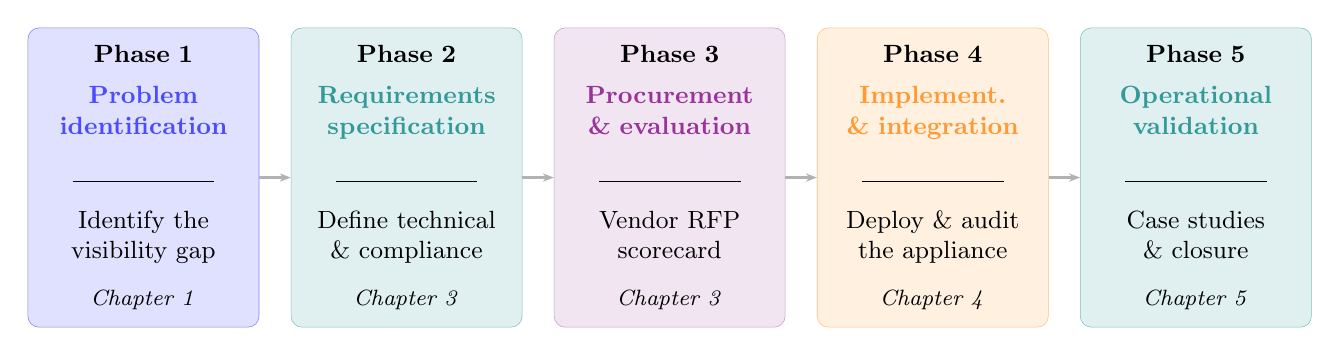
\begin{tikzpicture}[
    node distance = 0.4cm,
    box/.style = {
        rectangle,
        rounded corners=4pt,
        minimum width=2.6cm,
        minimum height=3.8cm,
        text centered,
        text width=2.7cm,
        draw,
        very thin,
        font=\small
    },
    ph1/.style = {box, fill=blue!12,   draw=blue!50},
    ph2/.style = {box, fill=teal!12,   draw=teal!50},
    ph3/.style = {box, fill=violet!10, draw=violet!40},
    ph4/.style = {box, fill=orange!12, draw=orange!50},
    ph5/.style = {box, fill=teal!12,   draw=teal!50},
    arrow/.style = {-{Stealth[length=4pt]}, thick, gray!60}
]
 
%% Phase nodes
\node[ph1] (p1) {
    \textbf{Phase 1}\\[4pt]
    \textcolor{blue!70}{\textbf{Problem}}\\
    \textcolor{blue!70}{\textbf{identification}}\\[6pt]
    \rule{1.8cm}{0.2pt}\\[6pt]
    Identify the\\visibility gap\\[6pt]
    \textit{\footnotesize Chapter 1}
};
 
\node[ph2, right=of p1] (p2) {
    \textbf{Phase 2}\\[4pt]
    \textcolor{teal!80}{\textbf{Requirements}}\\
    \textcolor{teal!80}{\textbf{specification}}\\[6pt]
    \rule{1.8cm}{0.2pt}\\[6pt]
    Define technical\\
    \& compliance\\[6pt]
    \textit{\footnotesize Chapter 3}
};
 
\node[ph3, right=of p2] (p3) {
    \textbf{Phase 3}\\[4pt]
    \textcolor{violet!80}{\textbf{Procurement}}\\
    \textcolor{violet!80}{\textbf{\& evaluation}}\\[6pt]
    \rule{1.8cm}{0.2pt}\\[6pt]
    Vendor RFP\\scorecard\\[6pt]
    \textit{\footnotesize Chapter 3}
};
 
\node[ph4, right=of p3] (p4) {
    \textbf{Phase 4}\\[4pt]
    \textcolor{orange!80}{\textbf{Implement.}}\\
    \textcolor{orange!80}{\textbf{\& integration}}\\[6pt]
    \rule{1.8cm}{0.2pt}\\[6pt]
    Deploy \& audit\\the appliance\\[6pt]
    \textit{\footnotesize Chapter 4}
};
 
\node[ph5, right=of p4] (p5) {
    \textbf{Phase 5}\\[4pt]
    \textcolor{teal!80}{\textbf{Operational}}\\
    \textcolor{teal!80}{\textbf{validation}}\\[6pt]
    \rule{1.8cm}{0.2pt}\\[6pt]
    Case studies\\
    \& closure\\[6pt]
    \textit{\footnotesize Chapter 5}
};
 
%% Arrows between phases
\draw[arrow] (p1.east) -- (p2.west);
\draw[arrow] (p2.east) -- (p3.west);
\draw[arrow] (p3.east) -- (p4.west);
\draw[arrow] (p4.east) -- (p5.west);
 
\end{tikzpicture}
\caption{IT Infrastructure Deployment Lifecycle Framework}
\label{fig:lifecycle}
\end{figure}






%_____________________________________________

\textbf{Phase 1 :} of the project lifecycle began with identifying Alpha Bank's core security issues. Over reliance on manually analyzing the bank's network traffic, having too few IT security personnel, and lacking any form of automated monitoring of their networks were just some of the challenges Alpha Bank faced. The main purpose of the project's first phase was to define a method to reduce the "Visibility Gap" within the bank's internal network by developing an AI-based Platform for Network Detection and Response (NDR) to enable automated, real-time threat detection.\\

\textbf{Phase 2:} Planning and Requirements Specification
Before acquiring a solution, it was important to define the specific parameters for the system that needed to be met. As part of this process, documentation of the technical, functional, and compliance requirements was completed. This included detailing technical specifications for the hardware performance baseline, including a minimum throughput of 5 Gbps with no packet loss, integration capability into the current Security Information and Event Management (SIEM) stack, and local data sovereignty compliance in accordance with Central Bank of Tunisia (BCT) regulations. \\

\textbf{Phase 3:} Procurement and Vendor Evaluation 
According to established specifications, Alpha Bank issued an RFP for global vendors and used a weighted selection matrix to objectively score the vendors based on criteria of accuracy (40\%), interoperability (20\%), privacy/compliance (20\%), and ease of use (20\%) for all vendors evaluated. The selection process resulted in the formal selection and justification of the Darktrace/NETWORK appliance.\\


\textbf{Phase 4:} Implementation and Configuration 
This phase involves putting into action, by physically implementing the project, the deployment of the approved acquisition of hardware within the Alpha Bank infrastructure and includes systematic installation, which will be done according to the following sequence of events: Installation of the appliances (racking); being connected (analysing cables) to the core switch; assigning static management IP address; synchronizing the NTP settings; and activating Secure Call-Home connectivity. Upon completion of the above tasks, diagnostic checks were performed to confirm ongoing traffic visibility.\\


\textbf{Phase 5:} Operational Integration and Handover
After Alpha Bank's appliance was successfully integrated into its production network, and after the completion of the initial baselining period, the final phase of this project focused on validating the operational effectiveness of the implemented solution against the functional requirements identified during Phase 2. The validation process was completed by reviewing and analyzing actual network incidents, which were detected by the system during the monitoring of an active production environment, using Darktrace Threat Visualizer and Cyber AI Analyst as primary investigative tools. Three case studies were reviewed and validated; false positive triage, Command and Control beaconing detection and a multi-device Domain Generation Algorithm campaign, which provided evidence-based validation that the solution meets the detection and analysis requirements laid out in the Call for Tenders. The engineering loop initiated during Phase 2 was officially closed by correlating each functional requirement with evidence produced in production to verify that the project's deployment objectives were achieved.

% ─────────────────────────────────────────────────────────────
\section{Conclusion}

The purpose of this chapter is to provide a complete overview of the work done throughout my internship with Alpha Bank. In addition, this chapter will outline the goals of my project as well as the major challenges encountered while working on the project. There has been a dramatic increase in the number and skill level of cyberattacks in recent years; therefore, securing network traffic has never been more important than it is today due to the everchanging nature of "threats" facing organizations globally. Consequently, the need to implement a robust and proactive monitoring solution, while once considered optional, is now a necessity. The recommended solution is an AI/ML - enhanced NDR platform, which will serve as a state-of-the-art security improvement to the bank's security measures. The next chapter will discuss the technical aspects of the implementation and deployment of the NDR platform.



% ============================================================
%  CHAPTER 2 — STATE OF THE ART
% ============================================================
\chapter{State of the Art}

\section{Introduction}

This chapter will focus on the key characteristics and challenges that motivate
the deployment of such a system. Then we’ll take a closer look at those technologies
logically correlated with what an NDR system does. Based on these technologies, we’ll
explore the key objectives and tasks that an NDR solution is required to accomplish, the
functional features it must provide, and the challenges you can encounter during the
preliminary evaluation, testing, and deployment phases.


%______________________________________________________________

\section{The Modern Network Threat Landscape}
To understand the necessity of behavioral network analysis, it is first imperative to examine how cyberattacks have evolved from opportunistic, isolated incidents into highly coordinated campaigns.

\subsection{Advanced Persistent Threats (APTs) and Dwell Time}
Modern threat actors are using methods similar to those employed by Advanced Persistent Threats (APTs). Unlike traditional ``smash-and-grab'' attacks, an APT is both covert and lasts long because they infiltrate a network and remain undetected for a long time (this is called the ``dwell time'')\cite{connectwise}. During this period, the attacker will methodically map the internal network topology, escalate their privileges, and set up command-and-control (C2) communications to their infrastructure. Because of the timeline of these actions (over several weeks or months), they will not typically create enough of a volume of activity to cross the thresholds that would activate a perimeter alarm (traditional).

\subsection{Lateral Movement and ``Living off the Land'' (LotL)}
Once an attacker is in the network, their first goal is to move laterally from where they compromised the network to target high-value servers (i.e., east-west traffic). To do this, today's attackers use ``Living off the Land'' (LotL) techniques to go undetected. LotL techniques exploit existing legitimate administrative tools that are already present in the attacked organization's environment, such as PowerShell, Windows Management Instrumentation (WMI), or authorized remote desktop protocols, instead of downloading identifiable malware. Because most of these tools will be whitelisted by any traditional security policy, there would be no distinction between the normal administrative use of the tools and the malicious use of those tools. So, when an attacker uses the tools to conduct an attack, it seamlessly blends in with typical administrative use of the tools.

\subsection{The Encryption Blind Spot}
Due to a growing interest in the protection of data throughout the world, there has been a lot of effort put into the use of cryptographic protocols like TLS 1.3. Encrypted traffic provides a layer of security for protecting data while it is being transmitted from one location to another. Unfortunately, however, this has created a large gap for defenders of networks. In most instances, malicious individuals who want to carry out attacks are taking advantage of encrypted tunnels in order for them to carry out malware delivery and exfiltration of data methods without detection from defenders. When using conventional deep packet inspection (DPI) firewalls, they cannot interpret the payload of any of the encrypted packets, therefore requiring extensive computing resources for SSL decryption, which comes with a high cost of reducing performance and increasing privacy concerns both for the network and the user. Consequently, modern security solutions need to include technologies that enable the analysis of both traffic patterns as well as metadata without needing to decrypt the individual packet payloads.

%______________________________________________________________

\section{The SOC Visibility Triad}
The Cyber Security Industry has adopted the ``SOC Visibility Triad'' to mitigate the limitations of standalone security tools following recommendations from research organizations like Gartner. To have comprehensive visibility, a mature Security Operations Center (SOC) must include three integrated and closely related aspects or pillars of visibility:
\begin{figure} [H]
    \centering
    \includegraphics[width=0.5\linewidth]{gartner.jpg}
    \caption{The SOC Visibility Triad \cite{gartner_soc_triad}}
    \label{fig:placeholder}
\end{figure}
\begin{itemize}
    \item \textbf{SIEM} ( Security Information \& Event Management system ) that provide visibility into logs and compliance data.
    \item \textbf{EDR} ( Endpoint Detection Response ) solution, provides detailed visibility of processes and file activity on user workstations and servers.
    \item \textbf{NDR} (Network Detection and Response): This aspect analyzes raw network traffic.
\end{itemize}

% ─────────────────────────────────────────────────────────────
\section{Architecture and Operation of an NDR}

This section focuses on how an NDR system is structured and how it operates. We begin
with a general overview of NDR, then examine the system's architecture in detail, and
finally explore the key operational processes including behavioral detection, automated
response, and security incident investigation.

\subsection{General Overview of an NDR}

\textbf{Network detection and response (NDR)} are a type of cybersecurity technology that goes beyond traditional signature-based methods for identifying cyber threats. With the help of artificial intelligence, machine learning, and analysing user behaviour, NDR solutions can also detect network anomalies, react to them when discovered, and make real-time decisions when there is a cyber threat.



\subsection{NDR Architecture}

A Network Detection and Response (NDR) system consists of different elements that work together to collect, analyze, interpret, and display network traffic to users in real-time under each of the four main components contained within the NDR system.

\begin{itemize}
  \item \textbf{A network data collection layer:} This layer is the most critical layer of any NDR in terms of building an NDR. This layer captures all of the data generated by the network and centralizes it. In order to collect this data, the layer uses technology methods like \textbf{port mirroring (SPAN)} to duplicate network activity and send it to the analysis (capture) layer. The data can consist of complete network packet information, metadata, device log data, flow analysis and communication data (IP addresses, ports, protocols etc.).

  \item \textbf{A behavioral analysis layer:} After the collection of network data, the behavioural analysis layer will create a thorough understanding of normality within the environment (i.e., who is communicating with whom at certain times using a certain volume of data and by what means and with which protocol). The behavioural analysis layer will create a baseline of normal behaviour over time, which may then be used as a reference point for identifying network behaviours that are outside of the established normal range.

  \item \textbf{An anomaly visualization layer:} functions as an interface between the technical detection engine and the security analyst. It translates complex detections into visually understandable formats (i.e., dashboards, dynamic charts, flow maps) so that analysts can easily understand and investigate detected threats.

  \item \textbf{Automated threat response modules:} enable automated response to suspicious or malicious activities as soon as they are detected. Responses are driven by pre-defined policies and artificial intelligence to produce responses for blocking a network flow, isolating infected computers, terminating sessions and sending alerts to the security staff for enhanced situational awareness.
\end{itemize}

%________________________________________________________________

\section{Behavioral Baselining and Machine Learning}
The Network Detection and Response (NDR) system utilizes Machine Learning (ML) in identifying what is considered ``normal'' activity in a network, instead of using specific known signatures of malicious activity that have already been established. The NDR uses, specifically:

\begin{itemize}
    \item \textbf{Unsupervised ML technology}: the NDR processes all of the Metadata collected from various sources (including IP Address, Port, Protocol, bytes sent, and interval times between packets) and applies a clustering algorithm to create a mathematical baseline of activity for each Device, User, and Subnet by developing and establishing baseline values against which activities can be measured.
    
    \item \textbf{Anomaly Detection}: After establishing this baseline, the system continuously compares real-time traffic against the historical model. An example of this is when a workstation that usually accesses internal web servers during normal business hours creates an SSH connection to sensitive database servers at 3:00 AM; this significant departure from established behavior generates an alert.

    \item \textbf{Encrypted Traffic Analytics}: Using machine learning algorithms, one can identify harmful behavior within encrypted network connections simply by analyzing the metadata (packet size, timing between packets, and outlier server certificate) of the packets passing through an encrypted tunnel; therefore, it is not necessary to have access to the actual content of the packets.
    
\end{itemize}




%---------------------------------------------------------------
\section{Comparative Analysis: NDR vs. Traditional Security Mechanisms}

To realize how important NDR is for today's architecture, it must be assessed against traditional security tools that have been the backbone of enterprise defenses.

\subsection{Intrusion Detection/Prevention Systems (IDS/IPS)}

Intrusion Detection Systems and Intrusion Prevention Systems use signature detection methods to detect possible intrusions or detect intrusions. These two types of systems have databases of known threat signatures (i.e., hashes or recognized malicious IP addresses or a specific byte sequence) and will block traffic that matches the corresponding signature. While traditional Intrusion Detection Systems (IDS) remain a foundational element of enterprise security perimeters, recent studies highlight their diminishing returns when operating in isolation \cite{diana2025}.

\textbf{The Limitation:} IDS and IPS are susceptible to ``Zero-Day'' attacks, which are new threats that do not yet possess a recognizable signature, as well as heavily obfuscated malware. Signature-based IDPS solutions are inherently reactive and severely limited when faced with zero-day exploits or advanced persistent threats (APTs) that utilize encrypted lateral movement \cite{abdulganiyu2023}.

\textbf{The NDR Advantage:} As opposed to dependent on static signatures like many other vendor solutions, NDR does not rely on static signatures but on using unsupervised machine learning techniques to identify what represents normal behavior in order to alert on the presence of anomalies (e.g., scanning of internal subnets by workstations) and thus detect new and zero-day threats which have the potential to bypass traditional IPS technologies. By applying unsupervised machine learning, the chosen NDR platform establishes behavioral baselines for all network devices, a method proven to be highly effective in identifying zero-day anomalous traffic without relying on static rules \cite{irabaruta2025}.

\subsection{Next-Generation Firewalls (NGFW)}

The objective of next generation firewalls is to secure the network perimeter (i.e., north-south or internet-to-internal traffic flow) by applying access control policies and conducting deep packet inspection between an internal network and the internet. Once an attacker has successfully bypassed a firewall (such as through a phishing email or compromised VPN credentials) the firewall provides minimal visibility into the lateral movement (i.e., east-west or internal-to-internal traffic flow) occurring within the network between servers/workstations.

\textbf{The NDR Advantage:} NDR technologies can be implemented as part of the core or central point within your network to monitor all internal East-West traffic through visibility solutions. Consequently, if an attacker breaches the perimeter, then any actions taken by the attacker inside the organization, referred to as ``internal propagation,'' can be rapidly identified using this architecture.

\subsection{Security Information \& Event Management (SIEM)} 

SIEM solutions assist security analysts by summarizing multiple log sources (endpoints, servers, firewalls) into one overall view of security events and activity on an organization's network/system. At a glance, analysts will have a central viewing location into all of the activity occurring on their respective organizations' networks.

\textbf{The Shortcomings of Log Data:} SIEMs rely on log data; log data has its inherent limitations. Log data may only include the information that an event has been programmed or configured to report by the system. Additionally, many advanced threats will manipulate, encrypt or disable the logging mechanisms on compromised systems to hide their activities.

\textbf{The NDR Advantage:} To mitigate the limitations of standalone security tools, modern network traffic analysis necessitates a dedicated NDR approach to provide definitive, ground-truth visibility \cite{ivanova2025}. When analyzing RAW Network Packets, your NDR provides the ``Ground Truth'' in Cybersecurity. Network Traffic cannot be Disabled or Tampered with by an Attacker. When Malware Uses a Network to Communicate, It Will Generate Packets. The NDR Will Detect These Packets.

\section{Conclusion}

The rapidly changing nature of cyber threats has made it necessary for organizations to shift from traditional reactive methods of responding to threats, such as using signatures of known threats, to a new proactive method which uses AI to create resilience. Network Detection and Response (NDR) analyzes raw network traffic, which contains all the necessary details for detecting and responding to sophisticated zero-day attacks. It also provides organizations with visibility of all internal systems and the ability to respond autonomously when an incident occurs.

With a solid understanding of NDR technology's theoretical and technical basis, we must now move from the academic to a real-world operation plan. As such, Chapter 3 is dedicated to the bank's formal Call for Tenders process. Within this chapter, we will define the architectural requirements of the organization, state our functional and technical requirements in detail and create evaluation criteria for acquiring and implementing the most appropriate NDR solution for use in a highly regulated financial industry.

%__________________________________________________________________________________
% CHAPTER 3 Needs Analysis & Solution Selection
%__________________________________________________________________________________

\chapter{Needs Analysis \& Solution Selection}

\section{Introduction}
This chapter is intended to connect the previous theoretical examination of Network Detection and Response (NDR) architecture with real world engineering practices. As such, it presents the formal call of tender (Needs Analysis and Technical Specifications) of the Alpha Bank solution. In this respect, this chapter provides strict functional, technical, compliance and hardware requirements that the required solution must meet , outlines all critical use cases associated with detection and includes an explicit weighted comparative analysis of all of the top vendors that responded to the tender. As such, it provides a basis on which to select the final solution.


\section{Project Objectives \& Scope}

In the framework of its proactive approach, Alpha Bank launched a tender for the acquisition
and implementation of a Network Threat Detection and Response (NDR) solution. The
solution must enable the bank to:

\begin{itemize}
  \item Detect cyber threats on the bank's network using Artificial Intelligence (AI),
    Machine Learning (ML), and data analysis.
  \item Detect anomalies and suspicious or malicious traffic on the network.
  \item Monitor network traffic in real-time and extract abnormal or suspicious connections.
  \item Generate automated responses to facilitate incident investigation activities.
  \item Use threat intelligence from inside and outside the bank to detect potential threats
    in network traffic, shareable with other security solutions within a converged security
    architecture.
  \item Provide an overview of the current security situation and threats to the network.
  \item Create a stream of security alerts indicating suspicious and potentially malicious
    network traffic.
  \item Act automatically and proactively using AI to prevent a cyber attack from
    succeeding.
\end{itemize}

The primary objective is to eliminate the \textbf{"Visibility Gap"} within Alpha Bank's
internal network. While existing tools (Firewalls, IDS/IPS) secure the perimeter, the NDR
must provide deep visibility into internal traffic to detect lateral movement and sophisticated
\textit{Zero-Day} threats.

%___________________________________________________
\section{Technical Specifications and Requirements}
To ensure the acquired solution aligns with the bank's rigorous security posture, a set of technical mandates was established.

% ──────────────────────────────────────────────────
\subsection{Functional Requirements (Detection \& Analysis)}

The solution must provide autonomous detection capabilities that do not rely on static rules
or historical signatures, as detailed in Table \ref{tab:functional}.

\captionsetup{singlelinecheck=false, justification=raggedright}
\renewcommand{\arraystretch}{1.4}

\begin{xltabular}{\textwidth}{c >{\bfseries\raggedright\arraybackslash}p{3.2cm} >{\raggedright\arraybackslash}X c}
    
    % --- FIRST PAGE HEADER ---
    \caption{Functional Requirements --- Detection \& Analysis}
    \label{tab:functional} \\
    \toprule
    \textbf{ID} & \textbf{Requirement} & \textbf{Specification} & \textbf{Priority} \\
    \midrule
    \endfirsthead
    
    % --- CONTINUED PAGE HEADER ---
    \multicolumn{4}{c}{} \\
    \toprule
    \textbf{ID} & \textbf{Requirement} & \textbf{Specification} & \textbf{Priority} \\
    \midrule
    \endhead
    
    % --- CONTINUED PAGE FOOTER ---
  
    
    % --- FINAL PAGE FOOTER ---
    \bottomrule
    \endlastfoot
    
    % --- TABLE DATA BEGINS HERE ---
    F1 & Behavioral Baselining &
    The establishment of distinct "Patterns of Life" for each user, device, and server within Alpha Bank using self-learning artificial intelligence will enable the solution to capture the unique behavioural baselines. & \critical \\
    
    F2 & Lateral Movement Detection &
    Monitoring East-West traffic (server-to-server) is critical for detecting attackers who have breached the perimeter and are moving laterally within the Alpha Bank network. & \critical \\
    
    F3 & MITRE ATT\&CK Mapping &
    All alerts will automatically be mapped to the MITRE ATT\&CK framework for the purpose of providing tactical context to SOC analysts. & \high \\
    
    F4 & Zero-Day Detection &
    The ability to detect zero-day attacks and new threats in real time without the use of signature-based detection methods will be a requirement of this solution. & \critical \\
    
    F5 & Botnet Detection &
    The system should be able to identify the various methods of botnet attacks as well as the command/control (C2) communications used between the botnet and its command/control server. & \high \\
    
    F6 & Behavioral Anomaly Detection &
    The system must be able to detect abnormal increases in user navigation activity compared to normal levels and any other behavioral abnormality. & \high \\
    
\end{xltabular}

% ──────────────────────────────────────────────────
\subsection{Technical \& Integration Requirements}

The NDR must act as a ``Sensor'' that enriches the bank's existing security ecosystem, as detailed in Table \ref{tab:technical}.

\captionsetup{singlelinecheck=false, justification=raggedright}
\renewcommand{\arraystretch}{1.4}

\begin{xltabular}{\textwidth}{c >{\bfseries\raggedright\arraybackslash}p{3.2cm} >{\raggedright\arraybackslash}X c}
    
    % --- FIRST PAGE HEADER ---
    \caption{Technical \& Integration Requirements}
    \label{tab:technical} \\
    \toprule
    \textbf{ID} & \textbf{Requirement} & \textbf{Specification} & \textbf{Priority} \\
    \midrule
    \endfirsthead
    
    % --- CONTINUED PAGE HEADER ---
    \multicolumn{4}{c}{} \\
    \toprule
    \textbf{ID} & \textbf{Requirement} & \textbf{Specification} & \textbf{Priority} \\
    \midrule
    \endhead
    
    % --- CONTINUED PAGE FOOTER ---
  
    
    % --- FINAL PAGE FOOTER ---
    \bottomrule
    \endlastfoot
    
    % --- TABLE DATA BEGINS HERE ---
    T1 & SOC/SIEM Integration &
    Native integration with the bank's SIEM (e.g., Splunk/QRadar) via API or Syslog to correlate network alerts with log data. & \critical \\
    
    T2 & EDR Interoperability &
    The ability to send and receive context from an Endpoint Detection and Response (EDR) System (CrowdStrike, etc.) is critical to achieving a single view of both host and network security. & \high \\
    
    T3 & Autonomous Response &
    The solution must include a ``Proportional Response'' capability (i.e. Surgical TCP Resets) so that the attack can be mitigated without disrupting overall banking services. & \high \\
    
    T4 & Performance \& Throughput &
    The hardware/virtual sensor must be able to provide a minimum throughput of 5 Gbps, while achieving 0\% packet loss. & \critical \\
    
    T5 & On-Premise Architecture &
    The solution must be fully deployable on-premise, without the need for any of its core functions to rely upon an external cloud service. & \critical \\
    
    T6 & IP Address Capacity &
    The system must be equipped to monitor a minimum of 5,000 IP addresses. & \critical \\
    
    T7 & Self-Contained Licensing &
    For the solution to work correctly, no other licenses, components, or external licensing need to be issued. In the event an operating system or database will be utilized in conjunction with the product, those license fees should be specified in the proposal for your bid. & \critical \\
    
\end{xltabular}

% ──────────────────────────────────────────────────
\subsection{Compliance \& Operational Requirements}

Alpha Bank, as a financial institution, is bound by certain regulations and privacy constraints.

\begin{description}[leftmargin=1.5cm, labelindent=0.5cm, style=nextline]
  \item[\textbf{Data Sovereignty}]
    All AI training and processing must occur locally/on-premises to ensure that any sensitive customer data remains in Alpha Bank’s environment.

  \item[\textbf{Auditability}]
    As part of its compliance with the requirements established by \textit{the Central Bank of Tunisia (BCT)}, the system is to provide a complete forensic audit trail (often referred to as "metadata" or "packet capture") for at least \textbf{30 days} as required in \textit{BCT Circular 2006-19}, that deals with the logging and traceability of administrative actions.

  \item[\textbf{Alert Triage Automation}]
    The approach should include an AI-analyst feature that consolidates numerous raw alarms into one security incident with the highest amount of fidelity and thus help to minimize fatigue among analysts. It should also be capable of changing the detection rules by defining different levels of sensitisations, as well as creating a standardised measure for every alarm collected and monitored using behavioural analysis and ongoing monitoring activities.

  \item[\textbf{False Positive Reduction}]
    The solution must facilitate configuration options that minimize false positive alerts and continuously enhance detection accuracy over time.

  \item[\textbf{Exceptions Management}]
    The provided solution will serve as a basis for creating and maintaining exception lists containing IP addresses, subnets, and/or valid domain names. In addition, the solution should provide the ability to adjust alert priority and/or the ability to disable specific alert types.
\end{description}

% ──────────────────────────────────────────────────
\section{Non-Functional \& Operational Requirements}

These ensure the solution is reliable and manageable by the bank's internal teams, as outlined in Table \ref{tab:nonfunctional}.

\captionsetup{singlelinecheck=false, justification=raggedright}
\renewcommand{\arraystretch}{1.4}

\begin{xltabular}{\textwidth}{c >{\bfseries\raggedright\arraybackslash}p{3cm} >{\raggedright\arraybackslash}X c}
    
    % --- FIRST PAGE HEADER ---
    \caption{Non-Functional \& Operational Requirements}
    \label{tab:nonfunctional} \\
    \toprule
    \textbf{ID} & \textbf{Requirement} & \textbf{Technical Specification} & \textbf{Priority} \\
    \midrule
    \endfirsthead
    
    % --- CONTINUED PAGE HEADER ---
    \multicolumn{4}{c}{} \\
    \toprule
    \textbf{ID} & \textbf{Requirement} & \textbf{Technical Specification} & \textbf{Priority} \\
    \midrule
    \endhead
    
    % --- CONTINUED PAGE FOOTER ---
  
    
    % --- FINAL PAGE FOOTER ---
    \bottomrule
    \endlastfoot
    
    % --- TABLE DATA BEGINS HERE ---
    NF1 & High Availability (HA) &
    The management console and sensors must support Failover/HA mode to ensure no security gaps during hardware failure. & \high \\
    
    NF2 & Role-Based Access (RBAC) &
    Integration with Active Directory (LDAP) to ensure only authorized Alpha Bank security analysts can view sensitive network captures. Multiple administration levels must be supported. & \high \\
    
    NF3 & Passive Deployment &
    Sensors must operate as passive listeners, adding no latency to network traffic and creating no single point of failure if overloaded or offline. & \critical \\
    
    NF4 & Adaptive Learning &
    The solution must use an adaptive model that evolves with the bank's information system and does not rely solely on knowledge bases, heuristics, or generic signatures. & \critical \\
    
\end{xltabular}

%___________________________________________________
\section{Infrastructure and Hardware Requirements}
This section outlines the physical constraints, deployment topology, and hardware required to support the NDR software without causing network degradation.

% ──────────────────────────────────────────────────
\subsection{Deployment Architecture (Physical Requirements)}

\begin{description}[leftmargin=1.5cm, labelindent=0.5cm, style=nextline]
  \item[\textbf{Traffic Capture Method}]
    The solution must support TAP (Test Access Point) and SPAN/Mirror port mirroring from
    the core switches (Cisco/Nexus/etc.). The solution must continuously analyze both
    north/south traffic crossing the bank's perimeter and east/west lateral traffic.

  \item[\textbf{Sensor Distribution}]
    Sensors must be deployable in the Main Data Center, the DR Site (Disaster Recovery),
    and the Internet Edge.

  \item[\textbf{Virtual Environment Support}]
    Capability to inspect traffic between Virtual Machines (VMware/Hyper-V) within the
    bank's private cloud.

    \subsection*{The Challenge of Virtual Network Visibility}
    Monitoring network traffic in an ordinary IT infrastructure is a relatively simple process because of the visible metallic wires and switches through which data travels. Nonetheless, the environment at Alpha Bank is a very heavy virtualization as shown in the fig \ref{fig:placeholder} so monitoring VM can become far more complex. Communication between VMs that are hosted on the same physical server is done via a virtual switch. Because all inter-VM traffic utilizes the server's software to pass between them, there is no physical network connection in this case (as all the traffic remains on the server). Therefore, traditional monitoring devices cannot detect this traffic.

    As a highly regulated financial institution, Alpha Bank faces a significant security risk with this scenario. The security team can monitor the flow of data into and out of the physical server, but they cannot see how data is being exchanged internally between the VMs. Alpha Bank needs complete visibility into all data flows in order to meet rigorous regulatory compliance requirements and to detect trends of cyber threats as they occur in real-time. By having complete visibility, Alpha Bank can also prevent an attacker from making any lateral movements within the organization that may not be obvious.

    \begin{figure}[H]
        \centering
        \captionsetup{justification=centering}
        \includegraphics[width=0.8\linewidth]{derk.PNG}
        \caption{Virtual Sensor With Virtual Switch}
        \label{fig:placeholder}
    \end{figure}
\end{description}

% ──────────────────────────────────────────────────

\subsection{Hardware Specifications}

To ensure the selected appliance could handle the bank's massive network traffic without bottlenecks, Alpha Bank's official Call for Tenders outlined strict minimum hardware specifications. The proposed solution had to meet or exceed the baselines detailed in Table~\ref{tab:hardware_specs}

\captionsetup{singlelinecheck=false, justification=raggedright}
\renewcommand{\arraystretch}{1.4}

\begin{xltabular}{\textwidth}{>{\bfseries\raggedright\arraybackslash}p{4.5cm} >{\raggedright\arraybackslash}p{4cm} >{\raggedright\arraybackslash}X}
    
    % --- FIRST PAGE HEADER ---
    \caption{Minimum Hardware Specifications}
    \label{tab:hardware_specs} \\
    \toprule
    \textbf{Component} & \textbf{Minimum Requirement} & \textbf{Notes} \\
    \midrule
    \endfirsthead
    
    % --- CONTINUED PAGE HEADER ---
    \multicolumn{3}{c}{} \\
    \toprule
    \textbf{Component} & \textbf{Minimum Requirement} & \textbf{Notes} \\
    \midrule
    \endhead
    
    % --- CONTINUED PAGE FOOTER ---
  
    
    % --- FINAL PAGE FOOTER ---
    \bottomrule
    \endlastfoot
    
    % --- TABLE DATA BEGINS HERE ---
    Form Factor          & 2U Rackmount, 19" rack       & \\
    CPU                  & Intel Xeon Gold              & \\
    Memory               & 256 GB                       & \\
    Storage              & 8 $\times$ 1.92 TB SSD RAID  & Total: 15.36 TB raw \\
    Operating System     & Latest version confirmed by editor & To be specified \\
    Maximum Throughput   & 5 Gbps                       & Without packet loss \\
    Connections/Minute   & 250,000                      & \\
    Admin Interface Ports & 1 $\times$ 10/100/1000 BASE-T & \\
    Remote Mgmt Ports    & 1 $\times$ 10/100/1000 BASE-T & \\
    Copper Analysis Ports & 2 $\times$ 10 GBASE-T        & \\
    SFP+ Analysis Ports  & 2 $\times$ 10Gbe/1Gbe SFP+   & Including SFP modules \\
    Power Supply         & Dual 1300W IEC 13C           & 100/240V, 50--60 Hz, Redundant \\
    Power Cords          & 2 $\times$ 3m IEC 320 C14--C13 \newline
                           2 $\times$ 3m IEC 320 C20--C13 14AWG & \\
    Certifications       & Safety, EMI certifications   & Required \\
    
\end{xltabular}

\noindent\textit{Note: Supported expansion modules must include 1G/10G SFP+ ports,
1G RJ45 1000 BASE-T ports, and 10G RJ45 BASE-T ports.}

%______________________________________________________
\subsection{Scalability \& Future-Proofing (2026 and Beyond)}

Alpha Bank's network will grow, and the NDR must grow with it. The solution must
demonstrate a clear roadmap for at least the next \textbf{5 years}.

\begin{description}[leftmargin=1.5cm, labelindent=0.5cm, style=nextline]
  \item[\textbf{OT/IoT Coverage}]
    The solution must be capable of expanding to monitor Operational Technology (OT),
    such as ATM networks and building management systems.

  \item[\textbf{Proactive Defense Integration}]
    Future capability to integrate with Attack Surface Management to identify externally
    exposed assets before they are exploited.

  \item[\textbf{Modular Expansion}]
    Ability to add specialized modules for Email or Cloud security if the bank decides to
    unify its entire security platform.
\end{description}

%____________________________________________________
\section{Operational Management \& Validation}
To ensure the solution is usable by the SOC team, strict reporting metrics and proof-of-concept validation tests were established.


%____________________________________________________
\subsection{Advanced Reporting \& Management Requirements}

The solution must provide actionable intelligence for all levels of the bank's security
hierarchy, from analysts to executives, as detailed in Table \ref{tab:reporting}.

\captionsetup{singlelinecheck=false, justification=raggedright}
\renewcommand{\arraystretch}{1.4}

\begin{xltabular}{\textwidth}{c >{\bfseries\raggedright\arraybackslash}p{3.2cm} >{\raggedright\arraybackslash}X c}
    
    % --- FIRST PAGE HEADER ---
    \caption{Advanced Reporting \& Management Requirements}
    \label{tab:reporting} \\
    \toprule
    \textbf{ID} & \textbf{Requirement} & \textbf{Technical Specification} & \textbf{Priority} \\
    \midrule
    \endfirsthead
    
    % --- CONTINUED PAGE HEADER ---
    \multicolumn{4}{c}{} \\
    \toprule
    \textbf{ID} & \textbf{Requirement} & \textbf{Technical Specification} & \textbf{Priority} \\
    \midrule
    \endhead
    
    % --- CONTINUED PAGE FOOTER ---
   
    
    % --- FINAL PAGE FOOTER ---
    \bottomrule
    \endlastfoot
    
    % --- TABLE DATA BEGINS HERE ---
    R1 & Threat Visualization &
    Must provide a real-time, dynamic map of the entire digital estate, showing all connections and potential attack paths. & \high \\
    
    R2 & Executive Dashboards &
    Capability to generate high-level reports for the RSSI showing ``Security Posture Trends'' and ``Risk Reduction'' metrics over time. & \medium \\
    
    R3 & AI-Powered Correlation &
    The solution must use an investigation engine (like a ``Cyber AI Analyst'') to automatically correlate benign events into single, understandable incidents. & \critical \\
    
    R4 & Standardized Exporting &
    The system must be able to extract and export forensic data and incident summaries into a standard format to meet regulatory reporting requirements to a BCT. & \high \\
    
    R5 & Retrospective Investigation &
    Must allow retrospective visualization of attack context to clearly identify machines, flows, protocols, and data volumes exchanged at the time the anomaly was detected. & \high \\
    
    R6 & Incident Reporting &
    Must offer incident reports and high-level statistics on real-time detection, autonomous response, frequently active models, devices with abnormal behavior, patch frequency, CVE distribution, and potential threats not covered by CVE. & \high \\
    
    R7 & MITRE ATT\&CK Coverage &
    Reports must include coverage of MITRE ATT\&CK framework showing devices with abnormal behavior by score, behavioral category, or MITRE attack technique. & \high \\
    
    R8 & System Health Alerts &
    The solution must generate alerts on system status and service health. & \medium \\
    
\end{xltabular}

% ──────────────────────────────────────────────────
\subsection{Mandatory Use Cases (Validation Criteria)}

The ideal NDR must be able to prove it can detect the following specific banking threats detailed in Table \ref{tab:usecases} during a trial (PoC):

\begin{table}[H]
  \centering
  \captionsetup{singlelinecheck=false, justification=raggedright}
  \caption{Mandatory Use Cases --- Validation Criteria}
  \label{tab:usecases}
  \renewcommand{\arraystretch}{1.5}
  \begin{tabularx}{\textwidth}{c >{\bfseries}p{4cm} X}
    \toprule
    \textbf{\#} & \textbf{Use Case} & \textbf{Description} \\
    \midrule
    1 & SWIFT/Payment Network Anomaly &
      Identify any unauthorized workstations that are trying to connect to SWIFT servers or Clearing servers via non-standard protocols. \\
    2 & Ransomware Propagation &
      Find a "Patient Zero" (for example, a laptop located in a remote branch) that is scanning for open SMB shares on the network as a sign of lateral movement towards spreading ransomware \\
    3 & Data Exfiltration via DNS &
      Find any compromised servers that are sending sensitive customer data out of the bank by tunneling through DNS queries, which are then used to bypass firewalls. \\
    4 & Rogue Device Detection &
      Automatically alert the SOC if a new, unauthorized hardware device (like a Raspberry
      Pi or rogue router) is plugged into a branch network. \\
    5 & Infected or Vulnerable Internal/External Machines &
      Detect risky traffic emanating from infected or vulnerable machines, both internal and
      external. \\
    \bottomrule
  \end{tabularx}
\end{table}




% ─────────────────────────────────────────────────────────────
\section{Solution Selection and Vendor Evaluation}

\subsection*{The Tender and Evaluation Process}

After developing the technical specifications, Alpha Bank began an \textbf{official request for proposals} from potential suppliers to find the best solution for the NDR project.Three global suppliers were chosen  as the finalists , those being \textbf{ Darktrace, ExtraHop (Reveal(x)), and Cisco (Secure Network Analytics)}. All three solutions were independently assessed against the bank's very high operational performance  and compliance standards before final selection. The results of that assessment appear in the following summary:

\begin{itemize}
    \item \textbf{Cisco Secure Network Analytics :} shows an excellent way to connect to what the Cisco equipment has to offer, but its detection engine relies mostly upon Netflow telemetry and previously known threat intelligence, therefore, it has difficulties providing Auto Signatureless-Zero Day detection as specified by the bank.

    \item \textbf{ExtraHop Reveal(x) :} has amazing line rate decryption and line rate throughput capabilities, yet it has a cloud-based architecture for processing machine learning which doesn't comply with the harsh requirements imposed by the Central Bank of Tunisia (BCT) regarding local data sovereignty and on-premise data processing.

    \item \textbf{Darktrace / NETWORK :} achieved the required throughput of 5Gbps and implemented completely unsupervised, self-learning AI. In addition, the Network enabled complete on-premise deployment and, therefore, met all of BCT’s compliance requirements.
\end{itemize}

\subsection{Final Evaluation Weighting (The ``Scorecard'')}

To provide an unbiased evaluation of the prospective suppliers aligned with Alpha Bank's priorities, a Weighted Selection Matrix has been developed. The scores applied to each of the suppliers for each of the criteria reflect my judgment based on the technical research done during the needs analysis process, the vendor documentation reviewed as a part of the RFP process, and the compliance requirements defined in Section 3.3.3. The score for each criterion is calculated based on how well it meets its weighted maximum, adding the cumulative scores of each supplier will result in a recommendation for the solution as detailed in Table \ref{tab:scorecard}.\\

The weighting scheme is based upon the primary security gap of Alpha Bank. As the existing security infrastructure employs Next-Generation Firewall (NGFW) and Intrusion Detection & Prevention Systems (IDPS) tools that satisfy basic compliance logging and integration with the bank’s networks, the most notable differentiator among the various vendors was their detection capabilities, specifically for behavioural anomalies with no known signatures. Therefore, the overall highest weighting of 40\% was designated to detection accuracy and equal weightings of 20\% were assigned to compliance, interoperability and ease of use to reflect their lower level of importance compared to the current security infrastructure.



\captionsetup{singlelinecheck=false, justification=raggedright}
\renewcommand{\arraystretch}{1.5}

\begin{xltabular}{\textwidth}{>{\raggedright\arraybackslash}p{3.5cm} c >{\centering\arraybackslash}X >{\centering\arraybackslash}X >{\centering\arraybackslash}X}
    
    % --- FIRST PAGE HEADER ---
    \caption{Evaluation matrix of proposed NDR solutions}
    \label{tab:scorecard} \\
    \toprule
    \textbf{Criterion} & \textbf{Weight} & \textbf{Darktrace} & \textbf{Cisco SNA} & \textbf{ExtraHop Reveal(x)} \\
    \midrule
    \endfirsthead
    

    % --- TABLE DATA BEGINS HERE ---
    Detection Accuracy & 40 pts & 37 / 40 & 26 / 40 & 31 / 40 \\
    
    Interoperability & 20 pts & 17 / 20 & 19 / 20 & 16 / 20 \\
    
    Privacy \& Compliance & 20 pts & 20 / 20 & 15 / 20 & 7 / 20 \\
    
    Operational Ease & 20 pts & 18 / 20 & 13 / 20 & 15 / 20 \\
    
    \midrule
    \textbf{Total} & \textbf{100 pts} & \textbf{92 / 100} & \textbf{73 / 100} & \textbf{69 / 100} \\
    
\end{xltabular}


\section*{Score Justifications}
\textbf{Detection Accuracy (40 pts)}
\begin{itemize}
    \item Darktrace — 37/40 Darktrace uses a completely autonomous, self-learning AI system to create unique Patterns of Life for all devices and users. The use of an entirely unsupervised AI system enables Darktrace to detect zero-day attacks, lateral movement, and command-and-control (C2) beacons with no reliance on signature-based techniques.
    Three points were withheld from the overall score to take into consideration the initial baseline period where there is a reduction in sensitivity of detection.

    \item Cisco Secure Network Analytics — 26/40 Cisco is largely reliant on netflow telemetry and already known threat intel. Requirement F4 requires zero-day detection with no signatures is a large challenge for Cisco. In addition, Cisco cannot provide any analysis of threats within encrypted traffic without additional decryption infrastructure.

    \item ExtraHop Reveal(x) — 31/40 ExtraHop shows good line-rate decryption and throughput performance, with solid machine-learning based detection systems. However, because their machine-learning condition has to be done in the cloud it depends on the availability of the cloud-based detection pipeline. Consequently there are latency and potential availability issues that do not allow production bank type environments to use this technology.
\end{itemize}

\noindent \textbf{Interoperability (20 pts)}
\begin{itemize}
    \item Darktrace — 17/20 has demonstrated integration capabilities via both a native API as well as via syslog to security incident and event management (SIEM) systems such as Splunk and/or QRadar. Darktrace also supports endpoint detection and response (EDR) interoperability with third-party products including but not limited to CrowdStrike. Three points have been deducted, however, due to the additional configuration efforts necessary for integrating Darktrace alerts into Alpha Bank’s current SOC workflow process.

    \item Cisco Secure Network Analytics — 19/20 Cisco had the highest interoperability score for their solution the second site across it is inherently integrated with the overall Cisco security ecosystem including Firepower, ISE, and SecureX. Institutions using Cisco network infrastructure would benefit from this inherent integration benefit.

    \item ExtraHop Reveal(x) — 16/20 ExtraHop shows standard APIs and Syslog can be easily integrated, but the dependence on a cloud-based architecture adds difficulty in interfacing with on-premise SIEM/firewall infrastructure. This added complexity reduces overall interoperability rating for this particular product within Alpha Bank's operating environment.
\end{itemize}


\noindent \textbf{Privacy \& Compliance (20 pts)}
\begin{itemize}
    \item Darktrace — 20/20 Darktrace achieved a remarkable perfect score in regards to the use of AI. All artificial intelligence training, data processing, and behavior analysis occur on their dedicated on-premises appliance; therefore, no raw network traffic or personal financial data will be sent outside of Alpha Bank's confines. This satisfies the requirements of the BCT Circular 2006-19 and the Requirement T5 regarding data sovereignty.

    \item Cisco Secure Network Analytics — 15/20 Cisco has developed a product that allows enterprises to deploy its own secure network analytics solution in an on-premise manner with local processing of the data and still meet the most basic requirement of sovereignty over their data. Cisco loses five (5) points because of its dependence on external threat feeds from third parties for intelligence. Therefore, Cisco must establish outbound connectivity to the cloud to process data received from those third-party data feeds at least on a periodic basis. Consequently, periodic outbound connections to the cloud must be explicitly whitelisted by third parties and documented in order to meet BCT compliance requirements.

    \item ExtraHop Reveal(x) — 7/20 ExtraHop's product utilizes cloud computing to perform its machine learning capabilities that result in sending the sensitive metadata from your network to a third-party cloud service for processing. The architecture of this uses an approach that fundamentally contradicts the requirements set forth by BCT Circular 2006-19 that requires on-premises processing of your data and sovereignty of your data within the region where you are located. This lack of compliance with those instructions significantly lowers the score on this criteria element.
\end{itemize}

\noindent \textbf{Operational Ease (20 pts)}
\begin{itemize}
    \item Darktrace — 18/20 Darktrace Cyber AI Analyst processes raw breaches to produce structured incidents autonomously, reducing the time taken by analysts to triage incidents by an estimated 92\%, according to Aite Group (Darktrace, 2023). The system provides analysts with an actionable interface via its Threat Visualizer, which significantly reduces the time it takes from receiving an alert to providing a complete incident timeline. Two points were deducted for the difficulty of understanding the AI's probabilistic scoring model.

    \item Cisco Secure Network Analytics — 13/20 Cisco's interface requires significant analyst expertise to navigate effectively, and its alert volume — driven by NetFlow-based detections — tends to be high, increasing triage workload. The absence of an autonomous investigation engine means analysts must manually correlate events across multiple views.

    \item ExtraHop Reveal(x) — 15/20 ExtraHop's Reveal(x) offers a relatively clean investigation interface and good alert prioritisation. However, its dependency on cloud processing for ML detections introduces response latency that is unsuitable for real-time SOC operations in a banking environment.
\end{itemize}




\subsection{Why Darktrace/NETWORK}

After a rigorous comparative analysis, \textbf{Darktrace/NETWORK} was selected as the
ideal solution for Alpha Bank, based on its unique ability to satisfy both the administrative
and advanced technical requirements of the bank.

\subsection*{Operational Added Value of the Selected Solution}

In addition to the comparative scorecard, Darktrace/NETWORK has a range of additional capabilities beyond the four evaluation criteria that will deliver considerable operational value to Alpha Bank's Security Operations Centre.\\

Cyber AI Analyst provides Darktrace with the ability to conduct autonomous investigations, which sets it apart from traditional NDR tools that produce large amounts of individual alerts and therefore require analysts to manually correlate those alerts together. Darktrace's Cyber AI Analyst, on the other hand, will automatically group related breaches (or model breaches) into consolidated, prioritized incidents that include a summary of the analysis generated by the AI. The ability to automate this portion of the process will allow Alpha Bank's Security Operations Centre to reduce the time it takes for analysts to triage breaches by 92\%, allowing the SOC to focus on strategic responses to incidents rather than on manually correlating events, which is particularly beneficial given the limited capacity of Alpha Bank's analysts.\\

Additionally, Darktrace has its platform designed to protect against new attack surfaces in future years. The platform is not limited to just monitoring network traffic and also includes email, cloud, and operational technology (OT) environments as part of a unified architecture. The Alpha Bank continues to develop and grow the bank's digital infrastructure and OT assets, like ATM networks, the same behavioral AI engine can be applied to monitor these additional environments without needing to enter into a separate procurement process.\\

Further, the platform’s credibility is further strengthened by independent third-party validation. Following thorough evaluations of the Detection Ability, Ability to Use the Platform, and Quality of Enterprise Support provided by Darktrace, independent financial technology research company Aite Group rated Darktrace 5 out of 5. The independent third-party validation from this research will also add to the selection process on top of the internal scorecard evaluation for computing.\\

Together, these components all evidence that Darktrace/NETWORK is the best solution to meet the two critical requirements of Alpha Bank based on its immediate security needs and its longer-term operational requirements, as evidenced by a total score of 92/100 from this scorecard evaluation.

% ─────────────────────────────────────────────────────────────
\section{Conclusion}

 This chapter gave a broad introduction to Network Detection and Response
(NDR) solutions by explaining how they operate, and outlined the process of
how a company selects an NDR vendor and solution via a tendering process. Next, the
chapter detailed the specific selection criteria based on which Darktrace became the
chosen solution. These selection criteria are the self-learning AI engine, the real-time
detection of abnormal behavior, and the visualization and in-depth investigation by the
3D interface features. Finally, an overview of Darktrace as an NDR solution was given.
Chapter 4 will go more in-depth by explaining how Darktrace is built in terms
of network sensors, behavioral analysis modules, and response interfaces. Next, a 3D
visualization of the network helps with the investigation of detected anomalies.
Moreover, the deployment process will be explained in more detail. What are the key
steps needed for acquiring and installing the software and devices of this specific
NDR solution and integrating it into the network environment n steps carried out to bring the solution into
operation within the organization.









































% ─────────────────────────────────────────────────────────────
% =============================================================================
%  CHAPTER 3 — SETTING UP THE DARKTRACE APPLIANCE
% =============================================================================
\chapter{Setting Up the Darktrace Appliance}

\section{Introduction}

A physical installment of Darktrace’s equipment was made at Alpha Bank through a Darktrace field engineer and collaboration with Alpha Bank’s internal infrastructure team. Instead of rehashing a typical vendor installation walkthrough, the chapter will take on more of an audit of deployment: In this case, it will perform systematic verification of Alpha Bank’s adherence (i.e., compliance) to the recommended engineering specifications for Darktrace's physical installations, as well as verifying if Alpha Bank’s chosen network configurations and integration decisions meet Alpha Bank’s security requirements stated in the Call For Tenders (Chapter 3).\\

Based on accepted standards in Engineering Management, when a new security appliance has been deployed, it is common to conduct an audit of that appliance using another engineer before the appliance can be transferred to the Operational group. This audit focuses on four major areas – the physical network connections, the configuration of the Management interface, the Call-Home Telemetry Channel, and the validation of post-deployment traffic visibility.

% ─────────────────────────────────────────────────────────────
\section{Physical Installation and Network Connectivity}

\subsection{Observed Physical Topology}

The Darktrace device was installed in a 2U rack mount configuration during its arrival at Alpha Bank's main data center. The installation matches the deployment architecture set out in the Call for Tender (Section 3.5.1) and also needs to have been installed in the Main Data Centre to capture the highest volume of internal east / west traffic.\\

The audit confirmed that the method for capturing traffic was SPAN/port mirroring from the bank core switch rather than via a passive network TAP. This design choice is worthy of further study since it represents a deliberate trade-off among cost, simplicity and resiliency.\\

\noindent \textbf{Why SPAN was selected over a hardware TAP}

A hardware Test Access Point (TAP), will passively and physically isolate all replicated data from the network. It does not create any risk of packet loss when there is a heavy load on the network. A TAP must be installed with dedicated physical cabling between the TAP device and the core switch. Therefore, a TAP will always require a separate piece of hardware to manage as well. For the initial deployment of a TAP at Alpha Bank, it was concluded that using SPAN (Switched Port Analyzer) mirroring would be sufficient for the following reasons:\\

The main switch at the bank can already facilitate dedicated SPAN sessions and has enough port capacity to send a complete copy of the traffic head over to the Darktrace analysis port.\\

The solution functions in a passive listening fashion (Requirement NF3), which means there is no added latency to the live traffic through the SPAN session, regardless of how it is implemented.\\

The use of SPAN-based deployments allows for easy addition of more VLANs or segments without needing to run new cable; this is particularly important because Alpha Bank plans to extend their monitoring reach beyond 2026 (Requirement T6).\\

The SPAN session has been set up so that all of the VLANs used for production are mirrored, so that none of the segments will be left out of the capture scope. This decision will ensure that the Darktrace appliance is receiving a full and accurate representation of Alpha Bank's entire internal network traffic as well as maximizing the amount of behavioural visibility that will be possible for the machine learning engine, while preventing any types of blind spots from occurring using a selective approach to VLANs.

\subsection{Interface Cabling and Port Configuration}

The Darktrace appliance comprises two distinct categories of physical interfaces, each designated for a specific function:\\

Darktrace provides users with multiple ways to access the Threat Visualizer web interface, the console application as well as completing any other administrative functions: via the Management Interface (1 Gbps copper RJ45). The Management Interface is connected to Alpha Bank's dedicated Administrative Network using standard CAT6 patch cables.\\

The analysis port (10G or 1G via SFP+) receives a mirror of the traffic on the production network over a core switch SPAN session. The 10-Gbps SFP+ is chosen as the preferred approach because it can support the extremely high bit rate associated with the SPAN session, which mirrors all production VLANs simultaneously—that is, over 1 Gbps during peak times in the banking industry.\\

The network access ports that have been verified as open according to Alpha Bank's internal firewall rules are outlined in Table ~\ref{tab:network-ports} below.


\begin{table}[H]
  \centering
  \captionsetup{singlelinecheck=false, justification=raggedright}
  \caption{Network Access Port Requirements}
  \label{tab:network-ports}
  \renewcommand{\arraystretch}{1.4}
  \begin{tabularx}{\textwidth}{X p{3.2cm} p{2.4cm} p{2.2cm}}
    \toprule
    \textbf{Connection} & \textbf{Port} & \textbf{Direction} & \textbf{Required?} \\
    \midrule
    Threat Visualizer and web configuration. Communication between master and probe/Unified View.
      & 443 (TCP) & Inbound & Required \\
    Console application and file transfer via SFTP
      & 22 (TCP) & Inbound & Required \\
    Network Time Protocol
      & 123 (UDP) & Outbound & Required \\
    Syslog ingestion of mapping data
      & Various & Inbound & Optional \\
    DNS querying
      & 53 (TCP \& UDP) & Outbound & Optional \\
    Scheduled Backups (SCP/SMB/S3)
      & 22, 445 or 443 (TCP) & Inbound & Optional \\
    Call-Home
      & 443 (TCP) & Outbound & Optional \\
    Remote management KVM
      & 80, 443, 7578 (TCP) & Inbound & Optional \\
    \bottomrule
  \end{tabularx}
\end{table}



\normalsize
\vspace{0.3cm}

\subsection{Syslog Input}

Data from syslog is ingested via several different port/protocol combinations. The choice of which to use will depend on the network environment, if the syslog sends are using common export formats, and whether or not the syslog data needs to traverse untrusted networks.

The configurations that are supported are detailed in Table ~\ref{tab:syslog-ports}.

\begin{table}[H]
  \centering
  \captionsetup{singlelinecheck=false, justification=raggedright}
  \caption{Syslog Input Port Configuration}
  \label{tab:syslog-ports}
  \renewcommand{\arraystretch}{1.4}
  \begin{tabularx}{\textwidth}{X p{3.2cm} p{2.4cm} p{2.5cm}}
    \toprule
    \textbf{Connection} & \textbf{Port} & \textbf{Direction} & \textbf{Encryption} \\
    \midrule
    Syslog input to standalone master or probe & 1514 (UDP or TCP) & Inbound & Unencrypted \\
    Syslog input to standalone master or probe & 6514 (TCP)        & Inbound & TLS / SSL \\
    Syslog input to Unified View               & 2514 (UDP or TCP) & Inbound & Unencrypted \\
    Syslog input to Unified View               & 7514 (TCP)        & Inbound & TLS / SSL \\
    \bottomrule
  \end{tabularx}
\end{table}

The default ingestion port can be altered in the host variables of the appliance
after configuration. Unused syslog ports can also be disabled if desired for
compliance purposes.

% ─────────────────────────────────────────────────────────────


% ─────────────────────────────────────────────────────────────
\section{Management Interface Configuration}

\subsection{Static IP Assignment}

Stable and predictable addressability is a basic requirement of any production security appliance. The Darktrace management interface has been statically assigned an IPv4 address within Alpha Bank’s dedicated management VLAN, as opposed to being assigned a DHCP addressed (Dynamic Host Configuration Protocol). This decision directly aligns with Requirement NF1 (High Availability) of the principles of Operational Continuity. If there was a failure or the DHCP server was reallocated during a maintenance window, a Darktrace appliance that had been allocated via DHCP could become unreachable from the Security Operations Center (SOC) precisely at the moment that an incident would need to be investigated.\\

The static assignment was created with the bank's internal default gateway and DNS server addresses so that the appliance can resolve internal host names. This is important to enrich device names. As seen in the Threat Visualizer, this is why internal servers have their fully qualified domain names in place of just showing their raw IP address.

\subsection{Time Synchronisation Strategy}

Having accurate time synchronization isn't only about convenience for NDR (Network Detection and Response) but is also crucial when it comes to ensuring the integrity of your investigation. The timestamps of each model breach, connection event, and Cyber AI Analyst investigation featured in Chapter 5 are only valid if they can be verified by using a common and consistent time reference. For instance, if the time between your Darktrace and your SIEM (Security Information and Event Management system) or Active Directory logs are out of sync by as little as a few seconds, any correlation between the two tools will be undependable; therefore, this could cause your evidence to be deemed invalid during a regulatory audit.\\

The Darktrace appliance has been set up to synchronize its time with a dedicated internal Network Time Protocol (NTP) server within the Alpha Bank infrastructure instead of using a public NTP server. This decision is deliberate; if an external NTP server were to be used, another outbound firewall rule would have to be added and the appliance would become dependent on the availability of internet connectivity. By using a dedicated internal NTP appliance, which then synchronizes itself with an external authoritative server for time information, the Darktrace appliance inherits access to a verifiable and dependable time reference that remains completely contained within the bank's network. The architecture employed by this configuration is consistent with the time synchronization provisions of BCT Circular 2006-19 related to critical security infrastructure.


% ─────────────────────────────────────────────────────────────
\section{Call-Home Telemetry Channel Configuration}

An outbound encrypted communication channel is established through the Call-Home feature from the local Darktrace instance to Darktrace's Threat Intelligence Network (TIN). This provides the appliance with ongoing updates from its machine learning models and emerging threat intelligence, as well as new model definitions without transferring any sensitive Alpha Bank traffic data off of the site. Thus, AI processing will take place entirely on site, satisfying Requirement T5 and complying with the data sovereignty requirement specified in Section 3.3.3.

\subsection{Security Constraint: Firewall Whitelisting}

The policy for the network security of Alpha Bank represents an explicit prohibition against unrestricted outbound internet access from any security appliance. This is consistent with the widespread industry practice of hardening all security appliances as part of an organization's standard operating procedure (SOP) in accordance with regulatory compliance requirements. An unrestricted outbound access configuration of an NDR appliance if compromised could act as a vector used to exfiltrate bank records from the organisation's system (internal network). To meet both the bank's operational requirement to access threat intelligence updates and to comply with a least privileged architecture, the bank has developed the following architecture:\\

Outbound TCP port 443 was allowed for the Alpha Bank Darktrace instance, so only the specific hostname assigned to Alpha Bank was allowed for outbound TCP port 443 access in the perimeter firewall instead of a broad-outbound rule for outbound TCP port 443 through the perimeter firewall. The Alpha Bank hostname is unique to each customer implementation and can be found in the appliance console under "Appliance Admin" -> "Call-Home" -> "Call-Home Configuration." Therefore, the firewall rule only allows TCP/443 outbound traffic from the management interface to the customer-dedicated endpoint for Alpha Bank; all other outbound HTTPS traffic originating from the management interface of the appliance will be blocked.\\

This strategy exemplifies the principle of least privilege at the network layer: the appliance is granted precisely the connectivity required for its operation, with no additional access permitted.

\subsection{Call-Home Validation}

Following the implementation of the firewall rules, the validation of the telemetry link was conducted through a three-step verification process:\\

DNS Resolution Test; The appliance console was used to confirm the Call-Home hostname resolves correctly to its assigned address using Alpha Bank's internal DNS. If this fails, it either means the DNS configuration is wrong, or there is no rule for that DNS server.\\

In order to validate whether the Firewall whitelist for the endpoint was correctly applied, an initiated TCP connection attempt from the appliance to the remote endpoint was made on Port 443. There were no proxies or content filtering intermediate devices which would potentially interfere with the establishment of the TCP connection.\\

The successful completion of the TLS handshake validated the trustworthiness of the Certificate Chain associated with the appliance, and proved the establishment of an end-to-end encrypted Channel.
% ─────────────────────────────────────────────────────────────
\section{Post-Deployment Validation}

\subsection{Traffic Ingestion Verification}

Having verified that physical, management configuration and telemetry connectivity are in place, the last phase of validation was to determine whether the Appliance was actively ingesting a complete and representative set of Alpha Banks’ internal network traffic. This last verification check is pivotal in the overall process of deploying NDR solutions; without observing traffic, an NDR solution cannot detect any threats regardless of how sophisticated the Artificial Intelligence models may be.\\

\noindent Validation of traffic ingestion was performed at two levels:


Interface-Level Bandwidth Statistics 
The live feed information coming from the Darktrace dashboard has been examined to confirm whether there is continuous traffic going through the analysis port (in this case, the analysis port is where I would expect to find ongoing analytics for the SPAN session). If there was insufficient bandwidth while conducting the analysis of the SPAN session to receive additional bandwidth on the analysis port, then, I would suspect that there was either a misconfiguration of the SPAN session, a broken cable, or possibly an incompatibility between the SFP+ module and the switch.

Statistics showed the core switch was replicating and sending live production traffic using the set up SPAN session and had evidence of no packets being lost or interfaces reaching saturation. This is an important note, as SPAN sessions on core switches that are very busy will, at times, lose mirrored packets when the internal fabric of the switch has a high load. The lack of packet loss also confirmed the Alpha Bank switch infrastructure has enough capacity to allow for the mirror session without any deterioration in production traffic being forwarded. \\

Asset Discovery Validation 
To confirm that Darktrace was properly identifying and classifying internal network devices through accurate parsing of the ingest network traffic, validation of Darktrace’s parsed data has also been performed against a device list in the Threat Visualizer (TV) using an expected device count as derived from IT assets (IP/MAC Address) records. If any significant discrepancies exist between these two totals this may mean there are missing VLANs from the SPAN session or errors with the subnet configuration within the Darktrace appliance device data.

Post-deployment validation confirmed that Darktrace successfully identified more than 1,000 internal devices across Alpha Bank’s monitored network segments. Device count aligns with bank’s network size, and confirms that the all-VLAN SPAN session provides complete coverage because there were no material gaps found during the audit of subnets.

\subsection{Initial Baselining Period}
The Darktrace appliance started its initial baseline phase, which is when picture an unsupervised machine learn model creates the pattern of life as defined in the F1 requirement. The system will not be sending any alerts for any aberrant activity during this phase but will accumulate enough statistical evidence to distinguish between true abnormal activity from normal fluctuations in the daily operation.\\

At Alpha Bank, the initial baselining period lasted approximately one month,
after which the SOC team began acting on Darktrace alerts as part of their
standard incident response workflow. This duration reflects the complexity of BH
Bank's network environment  over 1,000 devices across multiple VLANs and
network segments require a longer observation window to establish statistically
robust behavioural baselines than a simpler, more homogeneous network would.
The operational case studies presented in Chapter 5 were conducted after this
initial learning period had concluded, ensuring that the detection results reflect
a model fully calibrated to Alpha Bank's specific network environment  not a
generic out-of-the-box configuration.

% ─────────────────────────────────────────────────────────────
\section{Conclusion}

The purpose of this chapter is to describe an engineering integration strategy that was used to deploy the Darktrace NDR appliance at Alpha Bank. Key aspects of this deployment were the establishment of secure management access, the achievement of precise NTP time synchronization in order to ensure forensic accuracy, and the establishment of a hardened telemetry channel that provided for ongoing threat intelligence updates.\\

Validation of core traffic visibility confirmed that core switch traffic mirroring is operational. Because the appliance is fully integrated, securely managed, and receiving a full copy of all internal network traffic, foundational deployment is complete and the system is now set for conducting active network modeling and threat detection to meet the project's technical integration goals.

%___________________________________________________________
\chapter{Darktrace Threat Visualizer}

\section{Introduction}
Following the successful integration and configuration of the Darktrace appliance at Alpha Bank, the project was transitioned from deployment into operational validation. The objective of the NDR (Network Detection \& Response) solution is to proactively detect, investigate, and remediate cyber threats not captured by traditional defence mechanisms. This chapter provides evidence of the engineering success of the deployment through a demonstration of actual threat intelligence during operational phase. Specifically, using the Cyber AI Analyst, it provides an analysis of complex anomalies, separating from legitimate internal scans to fully functioning malicious Command and Control (C2) infections.

\section{ Overview of the Darktrace Threat Visualizer }
The Darktrace Threat Visualizer acts as the main way that security analysts at Alpha Bank will be engaging with the analytics output from the Darktrace system. This means that instead of simply displaying raw network telemetry, the dashboard will direct the analyst immediately to the highest priority incidents, offering AI-generated summaries, ranked by severity score, and a full catalog of all detected activity based on MITRE ATT\&CK Tactics. This design choice substantially reduces the mean time to triage, an analyst visiting the interface will not see a long list of thousands of low-level alerts; instead, they will view a clear and prioritized summary of the overall threat environment throughout the entire bank’s network.\\

Figure \ref{fig:1} The extent of the Alpha Bank implementation of Darktrace can be seen from data collected during the ongoing monitoring period. Over 5.8 billion network events were logged during this monitoring timeframe, with 2,501 breaches against the behavioural model detected by the system. The Cyber AI Analyst has created 30 defined structured and actionable incidents from these breaches, including 13 critical incidents. The breakdown of detections viewed via the dashboard against the MITRE ATT\&CK framework indicates that the highest risk detections were predominantly associated with the Command and Control tactic, with the 13 critical incidents correlated directly with the findings presented in Case Studies II and III of this chapter. The geographic mapping of network activity relative to the Alpha Bank location (Tunisia) clearly validates the installation into the production network of Alpha Bank. In addition, the Incident Carousel located at the bottom of the user interface displays 21 active (real-time) incidents, showing each incident with the corresponding device name(s), the number of incident events reported and device scopes associated with those incidents. Therefore, the analyst has instant access to situational awareness concerning current incidents without performing any manual searches.

\begin{figure}[H]
    \centering
    \captionsetup{justification=centering}
    \includegraphics[width=0.9\linewidth]{threat_visualizer.jpg}
    \caption{Darktrace Threat Visualizer interface}
    \label{fig:1}
\end{figure}


\section{Case Study I: Triage and Tuning of an Authorized Vulnerability 
Scanner}
\subsection{Detection Context}
The Darktrace appliance created a high-priority incident report for the Cyber AI Analyst's internal device, which is located in the Guest VLAN. This incident involved High-Risk Attack Paths and occurred between 11:50 and 11:55 UTC. The Cyber AI Analyst classified the associated model violations into two main categories, Internal Recon and Lateral Movement. Given that this was an unverified device accessing the Guest VLAN, the classified attacks pose a significant threat to the bank's internal infrastructure.\\

The internal server invest-carthago.client-domain.internal ([REDACTED IP]) was the main component of the observed activity, which is the web application hosted on an internal server and available to only the bank's internal LAN. Under Guest VLAN architecture, there is no method to gain unrestricted access to an internal application server, therefore this communications pattern is considered anomalous immediately from a network segmentation viewpoint.

\subsection{Model Breaches and Anomaly Analysis}
Within the five minutes summarised in Table~\ref{tab:model-breaches} below, the Darktrace model detected six separate model violations for [REDACTED IP]. Darktrace considers the activation of multiple independent behaviour-based models against the same device to be an event of Suspicious Network Scanning Activity. This combined alert is designed to identify devices that violate multiple scan-related models at the same time as violating at least one other, non-scan related model. Therefore, the simultaneous violation of these multiple models indicates a higher probability of malicious behaviour.

\captionsetup{singlelinecheck=false, justification=raggedright}
\renewcommand{\arraystretch}{1.4}

\begin{xltabular}{\textwidth}{>{\raggedright\arraybackslash}p{3.5cm} c c >{\raggedright\arraybackslash}X}
    
    % --- FIRST PAGE HEADER ---
    \caption{Darktrace Model Breaches for Device [REDACTED IP]}
    \label{tab:model-breaches} \\
    \toprule
    \textbf{Model Breach} & \textbf{Severity} & \textbf{Score} & \textbf{Description} \\
    \midrule
    \endfirsthead
    
    % --- CONTINUED PAGE HEADER ---
    
    % --- CONTINUED PAGE FOOTER ---
   
    % --- FINAL PAGE FOOTER ---
    \bottomrule
    \endlastfoot
    
    % --- TABLE DATA BEGINS HERE ---
    Device / Web Application Vulnerability Scanning & 
    \textbf{Critical} & 100 & 
    HTTP probing of invest-carthago.client-domain.internal on port 8180; Nikto URI signature (\texttt{/Trinity.txt.bak}) detected. \\
    
    Device / Port Scanning & 
    \textbf{Critical} & 100 & 
    8,802 TCP connections across 1,010 ports (range 1--65389) toward internal subnet. \\
    
    Device / Suspicious Network Scan Activity & 
    \textbf{Critical} & 100 & 
    Concurrent triggering of multiple independent scanning and non-scanning models on [REDACTED IP]. \\
    
    Device / Possible Brute-Force Activity & 
    \textbf{High} & 68 & 
    Repeated authentication attempts on port 8180 consistent with brute-force enumeration. \\
    
    Device / Unusual Administrative Connections & 
    \textbf{High} & -- & 
    East-west administrative connections toward invest-carthago.client-domain.internal flagged as lateral movement indicator. \\
    
    Device / Attack and Recon Tools & 
    \textbf{High} & -- & 
    OAST callback detected (nslookup injection toward oastify.com); Burp Collaborator pattern identified. \\
    
\end{xltabular}

Among the breaches noted above, the most impressive or "noteworthy" was the detection of an HTTP GET request using a URI that included "nice/ports/Trinity.txt.bak", which is indicative of the well-known Nikto open-source web application vulnerability scanning tool. Also, there was a detected callback to OAST (Out-of-band Application Security Testing) via an nslookup command injection against a domain registered with PortSwigger's Burp Collaborator platform (the domain is oastify.com). OAST techniques are often used in penetration testing to help identify server-side vulnerabilities (for example: Server-Side Request Forgery, Command injection, and XML External Entity injection) over an out-of-band communication channel. The AI Analyst summary for this specific event is illustrated in Figure~\ref{fig:inv1_web}.

\begin{figure}[H]
    \centering
    \captionsetup{justification=centering}
    \makebox[\textwidth][c]{\includegraphics[width=1.1\linewidth]{inv1.jpg}}
    \caption{AI Analyst Summary: Web Application Vulnerability Scan}
    \label{fig:inv1_web}
\end{figure}

A significant amount of TCP scanning activity is indicated by the data collected by the operating system, as detailed in the Port Scanning summary in Figure~\ref{fig:inv2_port}. The system created 8,802 connections to 1,010 different ports from 1 to 65,389. The ports that were targeted the most were: 21 (FTP), 22 (SSH), 23 (Telnet), 80 (HTTP), 135 (RPC), 389 (LDAP), 443 (HTTPS), 445 (SMB), 1,433 (MSSQL), 3,128 (Proxy), 3,306 (MySQL), 4,444 (Metasploit – default), 4,899 (Radmin), and 8,080 (HTTP – alternate). 

\begin{figure}[H]
    \centering
    \captionsetup{justification=centering}
    \makebox[\textwidth][c]{\includegraphics[width=1.1\linewidth]{inv2.jpg}}
    \caption{AI Analyst Summary: Port Scanning Breach}
    \label{fig:inv2_port}
\end{figure}

This activity aligns closely with what could be found in a full application and network vulnerability assessment. Following this extensive reconnaissance, Darktrace also detected anomalous east-west traffic, detailed in Figure~\ref{fig:inv3_admin} as an Unusual Administrative Connection. This activity further corroborates the profile of a comprehensive internal assessment and potential lateral movement.

\begin{figure}[H]
    \centering
    \captionsetup{justification=centering}
    \makebox[\textwidth][c]{\includegraphics[width=1.1\linewidth]{inv3.jpg}}
    \caption{AI Analyst Summary: Unusual Administrative Connection}
    \label{fig:inv3_admin}
\end{figure}

\subsection{Attack-Chain Reconstruction by the Cyber AI Analyst}

Using an autonomous methodology, the Cyber AI Analyst reassembled the stealthy behavioral sequences into a logical story about the attack (storyline), with an organization based on the Detect-Respond-Recover model. The analyst documented the chronological sequence of the attack, showing the temporal progression from Internal Reconnaissance through to Lateral Movement for device [REDACTED IP], as illustrated in Figure~\ref{fig:attack_chain}:

\begin{itemize}
    \item Web Application Vulnerability Scanning at 11:50:48 began the Internal Reconnaissance phase and was immediately followed by Port Scanning at 11:50:49.
    
    \item Unusual Administrative Connections 11:53:26, flagging east-west communication toward the application server invest-carthago.client-domain.internal.

    
    \item Identified as a potential follow-on concern, given the volume of information gathered during the reconnaissance phase.

\end{itemize}

\begin{figure}[H]
    \centering
    \captionsetup{justification=centering}
    \includegraphics[width=0.8\linewidth]{layer.jpg}
    \caption{AI Analyst Summary: Attack-Chain Reconstruction}
    \label{fig:attack_chain}
\end{figure}

During an assessment of web application vulnerabilities, the AI analyst noted that scans do not happen regularly enough to be scheduled vulnerability assessments; therefore, the security team should perform their own investigation. The port scan event exhibited what could be considered preparation for possible subversive and/or unauthorized internal activity. Unusual administrative connections resulted in a lateral movement alert; however, the AI analyst suggested that the lateral movement could be legitimate, or could be the result of a breach attempt because of compromised systems as well.

\subsection{Triage Investigation and Conclusion}
Once the incident report was received from Darktrace, a triage investigation was launched to determine if the exhibited behaviour was a valid security incident or if it was an approved operational activity. The originating IP address for the scan originating device ([REDACTED IP]) was compared against Alpha Bank’s registered infrastructure for conducting vulnerability assessments. The comparison confirmed that the IP address was located in the bank’s allocated subnet for the deployment of the Tenable vulnerability scanner. Verification was also performed on the type of tools and signatures that were detected: the Nikto web scanner, Burp Suite Collaborator (OAST) and the large range of ports scanned (1-65389) all match the tool profile associated with an approved penetration testing or vulnerability assessments operation. Also, based on the alert data that exhibited supplementary ICMP, TCP, and UDP scanning across internal subnets, the two Tenable connector IP addresses of [REDACTED IP] and [REDACTED IP] were identified as the origin of that scanning activity and thus confirmed that a coordinated, infrastructure-wide vulnerability scan was being performed at the same time as the detection of this activity.\\

In light of the facts established, it has been determined that this occurrence constituted a false positive based on the accurate and expected detection by Darktrace. Based upon the evidence reported on the device's established Pattern of Life, a behavioral deviation occurred, substantiating a requirements for further exploration into this event. The conclusion that the behaviour was approved does not indicate that there was an error in identifying this activity as such; instead, it demonstrates that the detection system's detection threshold has been properly set to identify also those internally-generated scanning activities that would occur from a well-calibrated Network Detection and Response (NDR) solution working in a complex financial setting.\\

The investigation was closed as an operational corrective measure in the Darktrace Interface, with an "investigation concluded" status. IP addresses identifying the Tenable scanner will be entered into an exception list for future alerts during scheduled scanning windows. The findings will prompt a series of recommendations to strengthen the network. These include the establishment of deny-by-default inter-VLAN ACLs to prevent Guest VLAN devices from communicating to internal application servers via flows that are not explicitly authorized and through Layer 3 and Layer 4 ACLs to restrict non-standard port access at the perimeter firewall.

\section{ Case Study II: Detection of a True Positive — SSL/HTTP 
Command and Control Beaconing}
\subsection{Detection Context and Threat Background}
C2 (Command and Control) beaconing is a major threat behaviour that Network Detection and Response (NDR) solutions are made to recognise. In C2 scenarios, malware installed on a compromised machine will periodically send automated communication to an external server under the control of an attacker to allow the operator to send commands, collect data or maintain an on-going connection with the compromised environment. C2 beaconing is characterised by periodic, low-volume connectivity from an infected machine to an external endpoint, and most of these connections will be encrypted (for example, utilising HTTPS over port 443). The communication patterns are intentionally designed to closely resemble legitimate web traffic, so as to not raise suspicion; therefore, signature-based detection mechanisms would not be able to identify the connection as malicious.\\

A Cyber AI Analyst detected a Critical-severity cyber event involving the Alpha Bank internal proxy device, proxybh2.client-domain.internal in November 2025, as captured by the Darktrace appliance. The event was classified within the Compromise/Beaconing Activity to External Rare under Darktrace's operational definitions. This classification is used when an internal device makes repeated attempts to connect to a defined external IP address, resulting in a "beacon score" (a numeric representation of the frequency of connections made) exceeding the "anomaly threshold" established in the Darktrace operational profile for that device. The incident received maximum possible criticality (100\%), which represents one of the highest-priority alerts registered by Darktrace during its operation.

\subsection{Cyber AI Analyst Autonomous Investigation}

When the Cyber AI Analyst discovered the first anomaly, it immediately launched an independent, multi-step investigation that did not rely on human intervention. The analysis proceeded according to the following steps:

\begin{itemize}
    \item Searching for recent unusual external connections from proxybh2.client-domain.internal.
    \item Discovered 48 unusual connections to 22 endpoints on port 443.
    \item Searching for further connections that may be related.
    \item Discovered 21,167 connections to 15 endpoints on port 443.
    \item Assessing this activity for signs of suspicious beaconing.
    \item Identified potentially suspicious beaconing to 2 endpoints on port 443.
\end{itemize}

The autonomous investigation chain removes the need for analyst involvement, condensing several hours of manual log correlation into a near-instantaneous, structured finding. The conclusion drawn by the AI Analyst found two specific external endpoints exhibiting statistically significant beaconing characteristics defined by the regularity, volume, and timing distribution of the connection data, as detailed in Figure~\ref{fig:inv4_beaconing}.

\begin{figure}[H]
    \centering
    \captionsetup{justification=centering}
    \includegraphics[width=0.8\linewidth]{inv4.jpg}
    \caption{AI Analyst Summary: Autonomous C2 Beaconing Investigation}
    \label{fig:inv4_beaconing}
\end{figure}

\subsection{Technical Analysis of Beaconing Behaviour}

Repeated connections to many external IP addresses via port 443 have been established through the model breach detail panel's confirmation of the IP address proxybh2.client-domain.internal, as shown in Figure~\ref{fig:beaconing_detail}. This type of beaconing behavior is commonly associated with the communication of unwanted or potentially malicious code, with the potential for connecting back to outside command and control (C2) servers. The investigation into whether the activity that occurred means malicious command and control operations or valid software is ongoing.

\begin{figure}[H]
    \centering
    \captionsetup{justification=centering}
    \makebox[\textwidth][c]{\includegraphics[width=1.1\linewidth]{proxy2.jpg}}
    \caption{Detection Detail: External Rare Beaconing}
    \label{fig:beaconing_detail}
\end{figure}

Regarding the "Compromise/Beaconing Activity to External Rare" model, the status of the model breach log shows that the investigation has been completed with the identifier "Investigation Concluded" and classified as an "External Connection," thus confirming that the anomalous communications are outbound. This is detailed in Figure~\ref{fig:beaconing_log}.

\begin{figure}[H]
    \centering
    \captionsetup{justification=centering}
    \makebox[\textwidth][c]{\includegraphics[width=1.1\linewidth]{model_alert_log.jpg}}
    \caption{Model Alert Log: C2 Beaconing Incident}
    \label{fig:beaconing_log}
\end{figure} 

The connection metadata tells us the source device, the destination port (443), and that the transport protocol is TCP, while the application data label indicates there is no user agent reported. The absence of the standard HTTP User-Agent header is a significant anomaly from the expected behaviour of legitimate web traffic created with a browser, which is consistent with the parameters for automated or malware-generated network communication.

\subsection{Escalation and Human-in-the-Loop Response}
A case study involving the scanner incident at Tenable was completed in a single investigation cycle, but the other C2 beaconing incident for the proxybh2.client-domain.internal (Alpha Bank) was sent to the Security Operations Center for an investigation and response by the Security Operations Center team. This distinction is not a limitation of the Darktrace platform, but instead, it reflects a deliberate and architecturally sound governance decision and is guided by internationally established incident response frameworks such as NIST SP 800-61 and ISO/IEC 27035.\\

Any self-contained containment activity that changes network connectivity in a financial institution subject to regulatory requirements, such as those set forth by the Central Bank of Tunisia (BCT) and the NIS Directive for essential service providers, must have approval from a human agent. Any mistake caused by an inappropriate containment action in a banking environment will cause immediate and major disruption. For example, if a valid server connection is initially interrupted due to containment, it can prevent payment processing, interfere with customer services, or make interbank settlement difficult. If there is strong evidence of a C2 incident affecting this bank, it is necessary to use an escalation process and not merely to take autonomous action. Intelligence will be provided by Darktrace, and the SOC will have the authority to take appropriate containment actions.\\

The NDR solution generates an organized, evidence-based report to guide SOC analysts through the escalation process. When a SOC analyst receives a n escalation, it is not in the form of a raw alert, but rather a complete report generated by Cyber AI Analysts. This complete report contains the a detailed timeline of detection, 21,167 correlated connections, 2 confirmed beacons that were communicating on port 443, a proxy server that had no user agent and then a history of Proxybh2.client-domain.internal's normal behavior, so that the SOC analyst can make an informed, timely and defendable decision in a regulated financial environment that requires adequate incident response capabilities.


\subsection{Current Investigation Status}
Currently, the Security Operations Center (SOC) team of Alpha Bank is investigating the C2 beaconing incident tied to proxybh2.client-domain.internal, which has been escalated and documented in the bank's Incident Response Workflow System. This continuing case is an example of how Alpha Bank's operations have successfully integrated the Network Detection and Response (NDR) solution into its operational security functions, as evidenced by an ongoing, live incident detected by Darktrace, resulting in corresponding security-related action/tresponse in the organization. Additionally, the NDR solution has met its primary operational goal of creating actionable information and enhancing the SOC's efforts to investigate.

\section{Case Study III: Multi-Device Command and Control / Suspicious Domain Campaign and HTTP Beaconing}
\subsection{Detection Context}
The final type of threat activity that was monitored during the operations period was a large number of devices found to be compromised. The scale and dispersion of these compromised devices makes them different from other cases of malware that have been tracked in the past. The pattern of multiple endpoints/PCs showing coordinated suspicious network activity simultaneously within a bank's internal network appears to be indicative of a single malware infection that has infiltrated a number of PCs/workstations simultaneously.\\

During the time of observation, Darktrace generated 6898 alerts in total under the category of Device/Suspicious Domain. The device interacts with an outside domain that has characteristics typically associated with malicious infrastructure, e.g., low reputation score, atypical TLD, and being made by techniques using Domain Generation Algorithm (DGA). The alert count is therefore significantly more than all other types of isolated endpoint compromises that also result in incidents.


\subsection{ Domain Analysis and DGA Characteristics}
Darktrace identified domains believed to be suspicious because of some of the common characteristics that can help differentiate between malicious command/control (C2) infrastructure and legitimate Internet locations. in particular, the use of a Domain Generation Algorithm (DGA) by malware developers allows them to use an algorithm to generate a large number of pseudo-random domain names, making it impossible for defenders to proactively stop C2 endpoint access every time. The incidents included domains with the following top-level domain (TLD) patterns, with .cyou (the largest category) being the overwhelming majority followed by .top, .rest, .live, .ml, .digital, .guru, and .ru, all of which are from low-cost domain registrars known to be widely used to generate malicious infrastructure that require very little identity verification to establish.\\

Some of the specific domains whose activity is being investigated by Darktrace include horizon-tn.com, barajind.top, seawow.pressyyahoo.rest, and airportinfo.live. Darktrace also correlated many of the domains they investigated with Possible HTTP Command and Control to Multiple Endpoints incidents. Therefore, it appears that, while the domain interactions observed did not occur as isolated browsing activity (i.e., someone specifically visits each site), the domain interactions occurred in an automated, repeating manner consistent with distributed command and control beacons established through HTTP requests.


\section{Multi-Device Correlation and Scope of Impact}

The most important indication of a compromise of the entire system in this incident was a cross-device correlation, which was performed by Darktrace on its own. The model titled Multiple Device Correlations / Multiple Device Triggering Same Model was triggered 33 times, indicating that multiple endpoints in the bank were independently using the same types of suspicious domains, and doing so within the same timeframes. When there is such a pattern, it indicates that there is a coordinated effort to spread malware, as infected hosts are all running the same Domain Generation Algorithm (DGA) and are attempting to communicate with their respective command and control (C2) infrastructure through the same generated domains.

Some of the many devices that participated in this campaign were: ag084pc50.client-domain.internal, aworkstations. The timing of alert clusterings also exhibited a remarkable level of consistency; for example, 10 model breach actions for the device ag084pc50.client-domain.internal were triggered between the hours of 08:00 and 08:12 on April 1, 2026. This twelve-minute period of unusual frequency of repeated contacts with suspicious domains indicates automated malware execution, rather than being consistent with standard patterns of human browsing. The resulting network of affected workstations and their connections to these common external suspicious endpoints is illustrated in the Incident Graph in Figure~\ref{fig:c2_graph}.

\begin{figure}[H]
    \centering
    \captionsetup{justification=centering}
    \makebox[\textwidth][c]{\includegraphics[width=1.1\linewidth]{3rd_case graphic.jpg}}
    \caption{Incident Graph: Multi-Device C2 Campaign}
    \label{fig:c2_graph}
\end{figure}

The Cyber AI Analyst created an investigative summary for a critical endpoint device (\#498803478.client-domain.internal). The device has exhibited several HTTP connections to a variety of unusual external endpoints while not containing user agent headers. This implies that the connections were established by at least one or more non-browser software processes. The analyst considered this behavior to represent Command and Control activity, as detailed in the detection summary in Figure~\ref{fig:c2_summary}.

\begin{figure}[H]
    \centering
    \captionsetup{justification=centering}
    \makebox[\textwidth][c]{\includegraphics[width=1.1\linewidth]{3er_case.jpg}}
    \caption{AI Analyst Summary: Multi-Device HTTP C2 Campaign}
    \label{fig:c2_summary}
\end{figure}

\section{MITRE ATT\&CK Framework Mapping}
To satisfy Functional Requirement F3 (section 3 of the Technical Manual), every alert generated by the Darktrace System must be methodically mapped to the MITRE ATT\&CK Framework, which provides both tactical/technical context to Security Operations Centre (SOC) analysts. Table \ref{tab:mitre} provides detailed mappings of the identified threat behaviours from all three operational incidents back to the corresponding MITRE ATT\&CK tactics and techniques.\\

The MITRE ATT\&CK framework is \cite{mitre_attack} the dominant global standard for organizing attacker behavior and has been developed by The MITRE Corporation and accepted by Cybersecurity teams worldwide. The Bh (Bank Host) SOC analysts may utilize the detection of network activity by mapping it back to the MITRE ATT\&CK framework in order to provide additional context about both the events which occurred at the network layer, and the phase of attack lifecycle indicated by the detected behaviours, as well as the next steps likely to be taken by attackers in order to complete an attack.

\renewcommand{\arraystretch}{1.6}

\begin{xltabular}{\textwidth}{>{\raggedright\arraybackslash}p{2.8cm} c >{\raggedright\arraybackslash}p{4.5cm} >{\raggedright\arraybackslash}X}
    
    % --- FIRST PAGE HEADER ---
    \caption{MITRE ATT\&CK framework mapping of threat behaviors detected by Darktrace during the operational validation period at Alpha Bank.}
    \label{tab:mitre} \\
    \toprule
    \textbf{Tactic} & \textbf{Tactic ID} & \textbf{Technique (ID)} & \textbf{Evidence Observed in Darktrace} \\
    \midrule
    \endfirsthead
    
    % --- CONTINUED PAGE HEADER ---
    \multicolumn{4}{c}{} \\
    \toprule
    \textbf{Tactic} & \textbf{Tactic ID} & \textbf{Technique (ID)} & \textbf{Evidence Observed in Darktrace} \\
    \midrule
    \endhead
    
    % --- CONTINUED PAGE FOOTER ---
  
    
    % --- FINAL PAGE FOOTER ---
    \bottomrule
    \endlastfoot
    
    % --- TABLE DATA BEGINS HERE ---
    Reconnaissance \cite{mitre_ta0043} & TA0043 & 
    Active Scanning: Vulnerability Scanning (T1595.002) & 
    8,802 TCP connections across 1,010 ports from [REDACTED IP]. Nikto scanner signature detected via HTTP GET to \texttt{/nice/ports/Trinity.txt.bak} URI. \\
    
    Discovery \cite{mitre_ta0007} & TA0007 & 
    Network Service Discovery (T1046) & 
    Port scan targeting ports 21, 22, 23, 80, 135, 389, 443, 445, 1433, 3128, 3306, 4444, 4899, 8080 --- key services profiled for lateral discovery. \\
    
    Lateral Movement \cite{mitre_ta0008} & TA0008 & 
    Remote Services: Web Protocols (T1021) & 
    Unusual Administrative Connections model breach flagged east-west communication from [REDACTED IP] toward invest-carthago.client-domain.internal on non-standard port 8180. \\
    
    Command \& Control \cite{mitre_ta0011} & TA0011 & 
    Application Layer Protocol: Web Protocols (T1071.001) & 
    SSL/HTTP Beacon model triggered 7 times at 100\% criticality. proxybh2.client-domain.internal established 21,167 connections to 15 external endpoints on port 443. \\
    
    Command \& Control \cite{mitre_ta0011} & TA0011 & 
    Dynamic Resolution: Domain Generation Algorithms (T1568.002) & 
    6,898 Device/Suspicious Domain alerts. Multiple devices contacted DGA-pattern TLDs (.cyou, .top, .rest, .live, .ml). 33 cross-device correlation events triggered. \\
    
    Exfiltration \cite{mitre_ta0010} & TA0010 & 
    Exfiltration Over C2 Channel (T1041) & 
    Internal Data Transfer metric matched on [REDACTED IP] (strength 56\%), correlated with beaconing activity suggesting potential data staging over established C2 channel. \\
    
\end{xltabular}

Four key phases of the MITRE ATT\&CK Kill Chain can be found within this analysis of incidents that have occurred during the operational period. The phases include: Reconnaissance (TA0043), Discovery (TA0007), Lateral Movement (TA0008), Command \& Control (TA0011), and there are indications that Exfiltration (TA0010) may also be present. This thorough coverage indicates that the existing NDR solution can detect adversarial activities through all completed attacks, which is something that Alpha Bank did not have with their original signature-based prevention controls.

\section{Assessment of the Cyber AI Analyst as an Autonomous Investigation Engine}

As demonstrated in the operational cases of this chapter, the Cyber AI Analyst has a measurable and continual capability that should be primary consideration when analysing: the automated, autonomous transformation of raw anomaly data into an organized, investigation-ready form of intelligence. This capability is a solution to the primary challenge identified in Chapter 1: the lack of dedicated security professionals employed by Alpha Bank precludes continuous, manual investigative process at the speed and volume needed to address today’s threat environment.\\

The operational usefulness of the AI Analysist can be clearly illustrated with the help of the C2 Beaconing Incident discussed in Case Study II. In this case, after a human analyst initiated an investigation based upon an alert they received from the initial model breach, the analyst would complete a number of tasks to identify the source device (along with its communication history), query their telemetry data base to identify all outbound connections from the previous time period, filter those outbound connections by destination rarity, port, and protocol, perform statistical tests to establish the periodicity of beaconing, correlate their results with their threat intelligence feed, and write a detailed report of their findings and recommendations. Based on established time benchmarks for this task at Security Operations Centres (SOC s), it generally takes between 45 minutes to several hours to complete. In contrast, the Cyber AI Analyst performed a functionally similar analysis where it was able to identify 48 anomalously connected devices located at 22 endpoints and expanded the total connection-count by a factor of 4,948 to 21,167 connections (at 15 of the same endpoints) while evaluating beacons and establishing that two had indications of being malicious – all accomplished almost instantaneously and without any manual interaction.\\

In Case Study III, the AI Analyst’s ability to correlate devices cross-device gave rise to an investigative advancement in which 33 Multiple Device Correlation Events are linked across five or more designated workstations. With each addition to agreed-upon endpoints, the complexity of the correlations grows exponentially. The Artificial Intelligence Analyst performed the correlation autonomously, giving the analyst a pre-synthesized view of the incident rather than multiple uncoordinated log entries.\\

In case study I, the output of an AI analyst acted as an analytical force multiplier. The AI Analyst produced a natural-language triage summary to evaluate the scanning behavior as likely not related to a scheduled vulnerability scan, as well as suggested proposing further investigation if the activity was deemed unexpected. This provided the investigating analyst with a structured basis which enabled significantly faster cross-referencing with existing Tenable scanner IP addresses. The overall determination was completed in minutes and a formal mechanism for recording the results was available through the systems’ interface, which improved the bank’s compliance audit trail.

\section{Requirements Validation / Closing the Engineering Loop}
The Call for Tenders (Chapter 3) serves as the contractual basis on which the success of this project will be evaluated. This section closes the engineering loop by matching the empirical data obtained from all 3 operational case studies against the mandatory use cases and functional requirement contained in the acquisition documents, as demonstrated in Table \ref{tab:validation} using a formal validation matrix.


\renewcommand{\arraystretch}{1.6} % You can keep your preferred 1.4 spacing now!

\begin{xltabular}{\textwidth}{c >{\raggedright\arraybackslash}p{3.8cm} >{\raggedright\arraybackslash}X c}
    
    % --- FIRST PAGE HEADER ---
    \caption{Requirements validation matrix mapping Chapter 3 functional requirements to operational evidence gathered during the Chapter 5 validation period.}
    \label{tab:validation} \\
    \toprule
    \textbf{Req. ID} & \textbf{Requirement} & \textbf{Evidence --- Chapter 5} & \textbf{Status} \\
    \midrule
    \endfirsthead
    
    % --- CONTINUED PAGE HEADER ---
    \multicolumn{4}{c}{} \\
    \toprule
    \textbf{Req. ID} & \textbf{Requirement} & \textbf{Evidence --- Chapter 5} & \textbf{Status} \\
    \midrule
    \endhead
    
    % --- CONTINUED PAGE FOOTER ---
   
    
    % --- FINAL PAGE FOOTER ---
    \bottomrule
    \endlastfoot
    
    % --- TABLE DATA BEGINS HERE ---
    F1 & Behavioral Baselining & 
    Darktrace established a unique Pattern of Life for device [REDACTED IP], enabling detection of scanning that deviated from its established behavioral baseline. & 
    {\textbf{Validated}} \\
    
    F2 & Lateral Movement Detection & 
    Unusual Administrative Connections model breach detected east-west movement from [REDACTED IP] toward invest-carthago.client-domain.internal, mapped to MITRE ATT\&CK Lateral Movement (TA0008). & 
    {\textbf{Validated}} \\
    
    F3 & MITRE ATT\&CK Mapping & 
    All model breaches automatically mapped to ATT\&CK tactics: Reconnaissance (TA0043), Discovery (TA0007), Lateral Movement (TA0008), Command \& Control (TA0011), Exfiltration (TA0010). & 
    {\textbf{Validated}} \\
    
    F4 & Zero-Day Detection & 
    C2 beaconing of proxybh2.client-domain.internal and DGA-domain campaign detected exclusively through behavioral anomaly analysis, with no known signature available at time of detection. & 
    {\textbf{Validated}} \\
    
    F5 & C2 Detection & 
    Seven SSL/HTTP Beacon alerts at 100\% criticality. AI Analyst correlated 21,167 connections to 15 external endpoints and confirmed suspicious beaconing to 2 endpoints. & 
    {\textbf{Validated}} \\
    
    F6 & Autonomous Investigation & 
    Cyber AI Analyst autonomously triaged the Tenable scanner incident, generated structured investigation summaries, proposed response actions, and formally closed the investigation. & 
    {\textbf{Validated}} \\
    
    F7 & Multi-Device Correlation & 
    Multiple Device Correlations model fired 33 times, linking simultaneous suspicious domain contacts across ag084pc50, ag000pc56, ag501-pc09, bh311poscaisse and others. & 
    {\textbf{Validated}} \\
    
\end{xltabular}

The validation matrix proves that all critical/high priority functional requirements outlined in the acquistion document have been met with regard to the operational monitoring period of the deployed DarkTrace NDR systems. The documented cases provide empirical evidence related to behavioral baselines, lateral movement detection, experienced mapping to the MITRE ATT\&CK framework, detection of zero day or signature-less threatenings, command/control (C2) beacons, independent AI driven investigations and multi-device correlation of threats; providing all the required capabilities outlined in the formal tender specifications.\\

The validation of Requirement F4 (Zero Day Detection) is important. The C2 Beaconing activity for proxybh2.client-domain.internal, and the DGA domain Campaign observed across multiple workstations, was detected only through behavioral anomaly analysis. There were no signatures for these specific threat patterns at the time of detection in any of Alpha Bank's current security tools. This shows that the NDR solution provides a unique and different layer of protection that other components of Alpha Bank's existing security infrastructure cannot duplicate.

\section{Conclusion}
The chapter validates the Darktrace NDR solution operationally at Alpha Bank through an in-depth analysis of three real incidents that occurred during the tool's first phase of production use. The case studies (1) case study of a false positive, (2) of a confirmed Command and Control beaconing, and (3) of a suspicious domain campaign across multiple devices show that the deployed solution operates as designed and provides a measurable security benefit to the real-time banking sector.\\

Through the case of the Tenable scanner, it was shown that the analyst team was able to determine the proper calibration of the scanner and its ability to differentiate between standard operational activities and legitimate threats. In the Command and Control (C2) beaconing situation with proxybh2.client-domain.internal, it was demonstrated that the NDR is capable of detecting sophisticated and encrypted outgoing malicious communications that bypass existing perimeter security measures of the bank. The suspicious campaign of multiple devices targeting their domain showed that the platform has an ability to identify distributed malware infections from a network perspective before any of the individual devices can be identified.\\

The results present clear evidence supporting the overall argument of this report that a behavioral AI driven Network Detection and Response system should provide a qualitatively enhanced security capability. The reason for this is that it uses network traffic as a true point of reference on which to obtain information; it cannot be altered due to either manual intervention or tampering with endpoint level logs; and it does not work from a list of known threats (signatures) and therefore has no limitation based on outdated indicators of compromise (IOCs). These three characteristics cannot be found in any aspect of the security technology stack currently used by Alpha Bank. Additionally, when examined using the MITRE ATT\&CK framework, this new NDR system demonstrates the potential for total visibility over the entire operational kill-chain based on the following actions being undertaken by an adversary: Reconnaissance, Discovery, Lateral Movement, Command and Control, and Exfiltration.\\

There are still some elements of the operation in flight as I write this; the investigation of C2 beaconing continues, and the SOC is continuing to enhance its behavioral models' understanding of Alpha Bank's unique network environment during the initial training effort. These are not limitations on the capabilities of the solution; they are simply an indication of the current operational status of a self-learning security platform as it evolves. The project has achieved its overall objective by giving Alpha Bank comprehensive visibility of its internal network traffic behaviorally informed, AI-enabled and already producing significant security intelligence and allowing for meaningful investigative activity in a production environment.


\chapter*{General Conclusion}
\addcontentsline{toc}{chapter}{General Conclusion}
\section*{Summary of the Work}

This document provides an overview of the complete lifecycle for acquiring and implementing a Network Detection and Response solution at a Tunisian financial institution known as Alpha Bank. Due to the complexity of the Alpha Bank network and compliance with the regulatory requirements established through BCT Circular 2006-19, it was necessary to improve the cybersecurity visibility posture of the organization.\\

Initially, an assessment of Alpha Bank's existing security perimeter revealed critical visibility limitations. While the bank relies on signature-based Intrusion Detection and Prevention Systems (IDPS) and Next-Generation Firewalls (NGFW), these perimeter defenses are ineffective at detecting the lateral movement of encrypted traffic, Advanced Persistent Threats (APTs), and zero-day behavioral anomalies. Consequently, it became evident that bridging this internal blind spot required a Network Detection and Response (NDR) platform powered by unsupervised machine learning rather than conventional rule-based systems.\\

To address these vulnerabilities, the identified security gaps were translated into a strict set of 20 functional, technical, compliance, and operational requirements. These criteria served as an objective evaluation matrix for three prospective vendors: Darktrace, Cisco Stealthwatch, and ExtraHop Reveal(x). Using a weighted scorecard prioritizing detection accuracy, regulatory compliance, interoperability, and operational ease, Darktrace/NETWORK was selected as the optimal solution that strictly adhered to Alpha Bank's data sovereignty and technical constraints.\\

During the deployment phase within Alpha Bank's primary data center, several key architectural decisions were executed to ensure seamless integration. These included utilizing SPAN port mirroring to maintain zero latency, allocating a static management IP, synchronizing with the bank's internal NTP infrastructure for accurate forensic logging, and securing the Call-Home telemetry channel via a least-privilege firewall whitelist. Post-deployment audits successfully validated that traffic ingestion was flawless, allowing the AI to commence its behavioral baselining.\\

Finally, the operational effectiveness of the solution was proven through real-world case studies on the live network. The NDR platform successfully distinguished authorized vulnerability scanning from malicious reconnaissance and autonomously correlated a complex, multi-device Command and Control (C2) campaign driven by Domain Generation Algorithms (DGA). By reducing 5.8 billion raw network events into just 30 structured, high-fidelity incidents (including 13 critical alerts), the deployment proved its immense value. The AI-driven NDR platform effectively eliminated alert fatigue, delivering actionable, prioritized intelligence to the SOC team and successfully securing the bank's digital estate.

\section*{Limitations}
This project was part of my internship for my Bachelor’s degree, and had a limited time frame in which to complete it. One thing to note is that during this period of time Darktrace’s RESPOND module, which can automatically quarantine devices or block connections on its own, was not turned on and therefore only worked in detection and alert mode and every response action required human validation. To turn on autonomous response comes with operational risk, such as containing false positives, and would take time for dedicated tuning and approval prior to being used in a live banking environment.

\section*{Future Perspectives}
Two strategic directions are proposed to enhance the NDR capability at Alpha Bank beyond this internship.\\

To begin with, Alpha Bank needs to expand its threat detection capabilities to include all cloud environments. Currently, Darktrace is only able to monitor the on-premise network traffic from Alpha Bank but does not have any capability to detect threats from services hosted within the cloud (SaaS) or through cloud providers. With the increasing reliance on both SaaS and cloud providers for critical operational services, Alpha Bank should use either Darktrace/CLOUD or another cloud-native network detection and response (NDR) to be able to apply the same method of determining the "normal" operational behavior to cloud workloads, in addition to monitoring hybrid traffic. This expansion will also enable Alpha Bank to enhance the auditability of its cloud data access, which is an area that traditional compliance solutions do not adequately address.\\

Secondly, integrate with ZTNA. Currently, the Darktrace deployment is used only for passive detection of threats; it does not enforce any type of access control. By linking threat signals from NDR with ZTNA, when a device is flagged for exhibiting suspicious activity, it can be automatically processed through policy enforcement. This integration will help provide a link between detection of incidents and the enforcement of those incidents while providing greater efficiency in incident response and reducing the time needed to contain incidents, which will be especially beneficial since Alpha Bank has a limited number of analysts.

\section*{Closing Remarks}
The project demonstrated how a modern financial institution can improve its ability to detect threats without impairing the production network, exposing sensitive data to processing in the cloud, or drowning the SOC team in too many alerts. The three incidents from Chapter 5 successfully corrected false positives, active C2 infection detected/escalated, and real time correlated multi device DGA campaign validate the effectiveness of the system on Alpha Bank's real network and solve real world problems.\\For a network handling thousands of daily financial transactions for Tunisian customers, this capability is essential.













\clearpage % Forces the page break so the TOC page number is accurate
\phantomsection % Ensures hyperref links point to the right place if you use clickable links
\addcontentsline{toc}{chapter}{\bibname} % Dynamically adds your "Bibliography" to the TOC
\renewcommand{\bibname}{Bibliography}
\nocite{*}
\bibliographystyle{IEEEtran}
\bibliography{bibliography}

\clearpage
\appendix 
\begin{appendices}
\addcontentsline{toc}{chapter}{Appendices}
\chapter*{Appendices}
\section*{Appendix A: Carbon Footprint Assessment — Internship (PFE)}

\textbf{1. Overall Carbon Balance }

\begin{table}[htbp]
\centering
\footnotesize % Reduces the font size one step further than \small
\setlength{\tabcolsep}{4pt} % Tightens horizontal spacing between columns
\renewcommand{\arraystretch}{1.2} % Tighter vertical padding for a more compact look

% Custom column alignments: L for left-aligned text with wrapping, C for centered
\newcolumntype{L}{>{\raggedright\arraybackslash}X}
\newcolumntype{C}{>{\centering\arraybackslash}X}

% Setting optimized custom widths for columns to minimize overall height
\begin{tabularx}{\textwidth}{>{\hsize=0.5\hsize}L >{\hsize=0.7\hsize}L >{\hsize=1.8\hsize}L >{\hsize=0.5\hsize}C >{\hsize=0.5\hsize}C}
\toprule
\textbf{Emission Source} & \textbf{Description} & \textbf{Calculation Details} & \textbf{Estimated Emissions (kg CO2e)} & \textbf{\% of Total} \\ 
\midrule

1. Transport & 
Round-trip commute (Home $\leftrightarrow$ Company) & 
Hybrid internship: 3 days/week on-site $\times$ 16 weeks = 48 days = 96 round trips. Distance: 9.6 km/trip. Mode of transport: bus (Tunis). ADEME emission factor: 0.089 kg CO2e/km. Total distance: 921.6 km $\times$ 0.089 = 82.02 kg CO2e. No international travel. & 
82.02 & 
60.0 \% \\ 
\addlinespace 

2. IT Equipment & 
Manufacturing of laptop, components, sensors... (internship: 4--6 months) & 
Laptop: manufacturing footprint of 300 kg CO2e, amortised over 48 months. 4-month internship: 300 $\times$ (4/48) = 25.00 kg CO2e. Smartphone (consultation): 50 kg CO2e $\times$ (4/36) = 5.56 kg CO2e. Total: 30.56 kg CO2e. & 
30.56 & 
22.3 \% \\ 
\addlinespace

3. Infrastructure \& Code & 
PC usage + Cloud server + Data transfer + Code execution & 
PC: 45 W $\times$ 8 h $\times$ 80 working days $\times$ 0.468 kg CO2e/kWh (Tunisia grid, IEA 2022) = 13.48 kg CO2e. Internet data transfer: 2 GB/day $\times$ 80 days = 160 GB $\times$ 0.06 kg CO2e/GB = 9.60 kg CO2e. No cloud usage (Darktrace on-premise). Total: 23.08 kg CO2e. & 
23.08 & 
16.9 \% \\ 
\addlinespace

4. Office Supplies & 
Report printing + stationery & 
Report printing: 2 copies $\times$ 80 pages = 160 pages A4. Emission factor: 0.006 kg CO2e/page (paper + printing). 160 $\times$ 0.006 = 0.96 kg CO2e. Stationery (pens, notebook): 0.50 kg CO2e. Total: 1.46 kg CO2e. & 
1.46 & 
1.1 \% \\ 
\midrule

% Total Row
\textbf{TOTAL} & & & \textbf{137.12 kg CO2e} & \textbf{100\%} \\ 
\bottomrule
\end{tabularx}

\vspace{0.2cm}
\raggedright
\footnotesize \textbf{* Calculation Details:} Intermediate results for each emission category are presented in the corresponding column.
\caption{Carbon Footprint Analysis Breakdown}
\label{tab:carbon_analysis}
\end{table}\\

\noindent\textbf{2. Improvement Proposals}\\
How to reduce the carbon footprint for future projects?
\begin{enumerate}
    \item \textbf{Prioritize remote work}:Reduce on-site presence from 3 days to just 1 day per week, 
working remotely for the remaining 4 days. This would significantly cut commuting 
emissions, which currently account for 60.0\% of the total footprint.
    \item \textbf{Digital eco-design}:Enable automatic PC sleep mode, limit unnecessary downloads, 
and prefer online reading over printing documents. 
    \item \textbf{Reduce printing}:Submit the final report in digital format; if printing is unavoidable, use 
recycled paper and limit the number of copies. 
    \item \textbf{Future cloud projects}:Select cloud providers powered by renewable energy (e.g. OVH 
Green, AWS EU) and optimize code to minimize server requests and data transfers.
\end{enumerate}
\end{appendices}
\end{document}